\chapter{Fitting}
\bichaptertitle{拟合}

\audiencebox{Staunch systems trader}{This entire chapter is about using data to create the
trading rules used by staunch systematic traders. It is not necessary reading if you are
going to use my framework to make discretionary forecasts as a semi-automatic trader or
without any rules at all as an asset allocating investor.\par\medskip
坚定的系统化交易者\par\medskip
整章都在讨论如何利用数据来创建坚定系统化交易者所使用的交易规则。
如果你打算作为半自动交易者在框架中使用主观预测，
或者作为资产配置型投资者根本不使用交易规则，
那么这章并不是必读内容。}

\noindent\textsc{A decision to run a systematic trading system means you have to select one
or more trading rules and discard others as being unworthy.} This process is often called
fitting. Given our human tendency to be overconfident this procedure is fraught with
danger. You need to beware of over-fitting:\footnote{Another common term for this is curve
fitting.\par 另一个常见术语是 curve fitting（曲线拟合）。} selecting a set of trading rules that fit past data too well and which are unlikely
to make money in the future.

\noindent\textbf{一旦你决定运行一套系统化交易系统，你就必须从若干交易规则中做出选择，并把其他规则淘汰掉。}
这个过程通常被称为“拟合”。由于人类天生倾向于过度自信，这个过程充满风险。
你必须警惕过拟合：也就是挑出一组对过去数据拟合得过于完美、
但在未来不太可能继续赚钱的交易规则。

\section*{Chapter overview}
\phantomsection
\addcontentsline{toc}{section}{Chapter overview}
\bisectiontitle{本章概览}

\begin{tabularx}{\textwidth}{@{}p{0.34\textwidth}Y@{}}
\textbf{The perils of over-fitting} & The dangers of trying to selectively choose and fit rules
based on past data. \\
\textbf{Effective fitting} & Steps you must follow if you insist on fitting your trading rules. \\
\textbf{How I choose my rules} & The process I use to avoid fitting almost entirely. \\
\end{tabularx}

\medskip

\begin{tabularx}{\textwidth}{@{}p{0.34\textwidth}Y@{}}
\textbf{过拟合的危险} & 试图基于过去数据选择并拟合规则时会遇到的风险。 \\
\textbf{有效拟合} & 如果你坚持要拟合交易规则，就必须遵循哪些步骤。 \\
\textbf{我如何选择规则} & 我用来几乎完全避开拟合的方法。 \\
\end{tabularx}

\section*{The perils of over-fitting}
\phantomsection
\addcontentsline{toc}{section}{The perils of over-fitting}
\bisectiontitle{过拟合的危险}

\subsection*{The 50 model kid}
\bisubsectiontitle{“50 个模型的小子”}

Shortly after leaving the hedge fund industry, I began discussions about consulting, and
managing some capital, for Aqueduct Capital,\footnote{All names have been changed to
protect the ignorant.} a local proprietary trading firm. The office contained the usual
mixture of grizzled ex-LIFFE traders and naive youths, all day trading a handful of futures
contracts. But the boss was particularly proud of his quantitative team which consisted of
a couple of 20-somethings toting PCs running an off-the-shelf back-testing software
package.

离开对冲基金行业不久之后，我曾和一家本地自营交易公司 Aqueduct Capital 讨论过顾问合作与资金管理的事情。那间办公室里有一种典型混搭：
既有饱经风霜的前 LIFFE 老交易员，也有天真的年轻人，大家整天都在交易少数几种期货合约。
而老板最自豪的，是他手下那支“量化团队”：
两个二十出头的年轻人，抱着电脑，运行现成的回测软件。

\begin{quote}
``This is Joe. He's only been here a month and he's already come up with 50 new trading
rules that are profitable in back-tests!'' exclaimed the boss.

``Yes, this software is amazing. It can automatically test hundreds of rules a day,'' added
Joe.
\end{quote}

\begin{quote}
“这是 Joe。他才来一个月，就已经搞出了 50 条在回测里赚钱的新交易规则！”老板兴奋地介绍。

“对，这软件太神了。它一天能自动测试几百条规则。” Joe 也补充道。
\end{quote}

I managed to keep a straight face and replied as diplomatically as I could, ``Well I am sure
some of them will work.''

我努力绷住脸，只能尽量委婉地回答：“嗯，我相信其中总会有几条能行吧。”

Inevitably the joint venture discussions then broke down, which was fortunate as the firm
was liquidated a few months later. The discovery of apparently profitable rules sifted from
thousands of possibilities is an incredibly dangerous approach, for reasons that will
become apparent in the rest of the chapter.

后来合作讨论果然无疾而终，而这其实是件幸事，因为几个月后那家公司就被清算了。
从成千上万种可能性里筛出那些“看起来盈利”的规则，本质上是一种极其危险的方法，
而本章后面会逐步揭示原因。

\subsection*{Ideas first testing for rules and variations}
\bisubsectiontitle{先有想法，再测试规则与变体}

Before understanding why Joe was on the wrong path you need to be clear on what fitting
actually involves. I'm going to restrict my attention in this chapter to the ideas first
method that I introduced in chapter two. You already know that I prefer the ideas first
approach, but the reason I use it here is because it's much easier to explain and understand
how to avoid over-fitting, than with the alternative of data first.

在理解 Joe 为什么走偏之前，你得先弄清楚“拟合”到底包括哪些步骤。本章里我只讨论第二章中引入过的“先有想法”方法。
你已经知道我偏好想法优先，但我在这里使用它还有一个现实原因：
相比“数据优先”，它更容易解释，也更容易说明如何避免过拟合。

The fitting process is going to involve selecting one or more trading rules from a list of
candidates, each based on a brilliant idea. Let's look at a contrived example, but beware
this is not a rule I would recommend using. The basic hypothesis is that the British
pound/US dollar currency rate seems to move in ranges as figure 6 shows. You might
think that buying pounds if they're 5\% below their average over the last year, and selling
at 5\% above, is a good strategy. This is an example of a mean reversion rule.

在这种流程里，你会先有一个想法，然后从若干候选规则中选出一条或几条来测试。比如，一个刻意构造的例子：
假设英镑兑美元汇率看起来常在一个区间里波动
（如图 6 所示），
于是你提出一条均值回归规则：
当英镑价格低于过去一年平均值 5\% 时买入，
高于平均值 5\% 时卖出。

You would now test this initial rule on historical data and look at how it performs and
behaves. At this stage if the rule is unpromising you can drop it and move on to the next
idea. If you like it enough you can proceed to the next stage which I call calibration,
although it's possible and often desirable to just stick with the initial version.

接着，你会用历史数据去测试这条初始规则，看它的表现和行为是否靠谱。
如果它不行，就放弃，去下一个想法；
如果它看起来还不错，你就进入下一步，我称之为“校准”
（calibration），
尽管很多时候，保留最初版本本身就是更好的做法。

\begin{figure}[htbp]
  \centering
  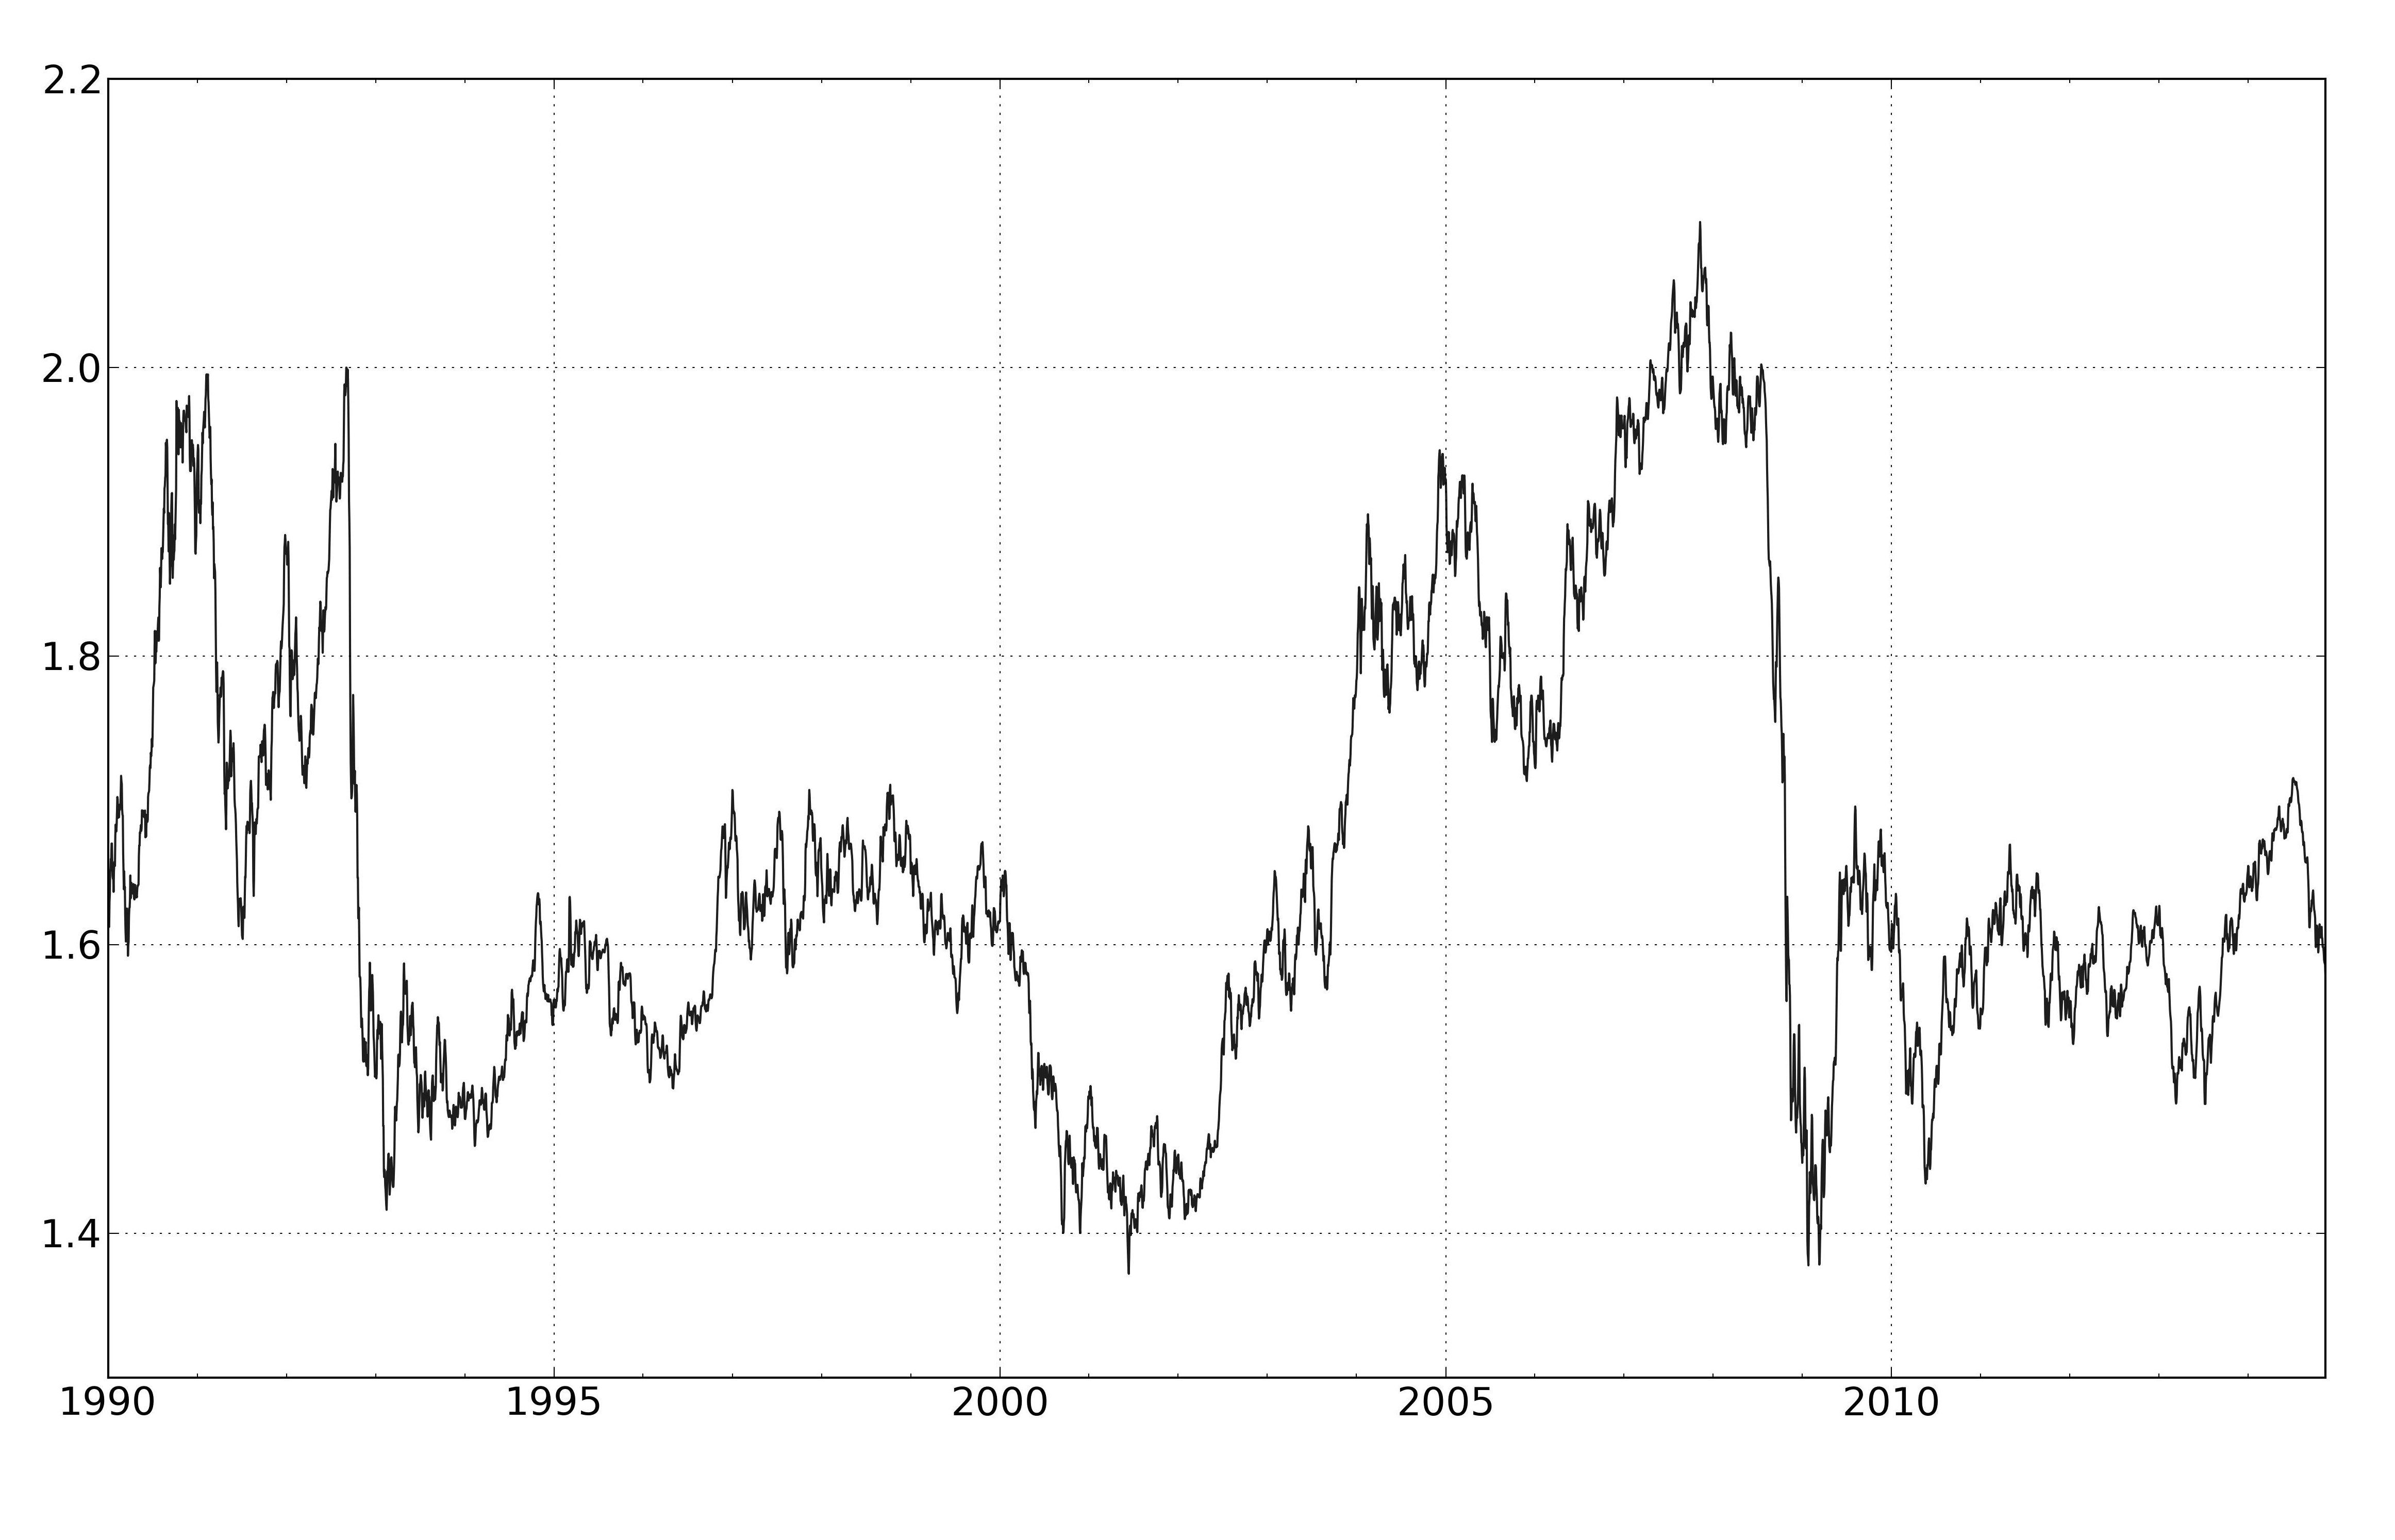
\includegraphics[width=\textwidth]{figures/raw/img-006.png}
  \caption{GBP vs USD exchange rate.\\
  英镑兑美元汇率。}
\end{figure}

During calibration you examine some variations on the basic trading rule. In the simple
example you could test the original range of plus or minus 5\% against alternatives such as
3\%, 6\% or 10\%; or you can compare the current price against the average price over the
last year, or week, or two years and so on. Usually you would choose the most profitable
rule using a performance measure like the Sharpe ratio. Calibration can also be used --- as
I will show later in the book --- to find rules which behave in a given way, such as trading
at a given speed. You can then decide which variation, or variations, to keep.

所谓校准，就是测试这条基本规则的一些变体。
在上面这个简单例子中，你可以测试 ±5\% 的阈值，也可以试试 3\%、6\%、10\%；
或者把“过去一年的平均价格”改成“过去一周”或“两年”的平均价格。
通常，人们会用夏普比率之类的绩效指标来挑出最赚钱的版本。
校准也可以被用来找出某种特定行为特征的规则
--- 比如交易速度达到某个水平的规则。

Once you have chosen a portfolio of trading rules and variations you need to decide how
to allocate your capital amongst them. Portfolio allocation decisions like this are the
subject of the next chapter. For the moment it's worth noting that a poor variation can be
rejected out of hand, or given a relatively small allocation in the overall system.

一旦你选定了一组交易规则和变体，下一步就是决定如何在它们之间分配资本。
这个“组合配置”问题，会在下一章展开。
这里你只需要记住一点：
一个表现差的变体，可以被彻底丢弃，
也可以只是被赋予一个较小的配置。

What if you want to use data first methods? Then you will need to be sufficiently expert to
apply the principles in this chapter with your own preferred tools.\footnote{The main
danger of the data first process is that you allow too many degrees of freedom. (I will not
be defining this term since anyone using a data first approach ought to understand it
already. If you don't you're in trouble!) Whereas the danger of ideas first is that you test
too many ideas, or variations of ideas, until you find one (or 50!) that work. Either
approach can result in over-fitted trading rules which look great in back-test but
underperform once actually trading.} You should not use a data first method for which
you don't have any deep understanding. I strongly suggest that you do not use a method
blindly, just because it came packaged with some back-testing software.

如果你坚持要用“数据优先”方法，那么你就必须具备足够的专业能力，
能把本章的原则真正应用到你的工具上。
绝对不要因为某种方法被打包进某个回测软件里，就不假思索地照单全收。

Before we continue here's a final note of caution about ideas first testing. Any worthy
trading systems designer will know their history, have read all the right textbooks and be
aware of what other people trade. You could end up testing only ideas that you already
know will work, which is a form of implicit over-fitting. As a result no matter how careful
you are with the subsequent fitting process your back-tested Sharpe ratios will probably still
be overstated --- beware overconfidence!

最后，还要提醒一点：即便你采用“想法优先”，也并不意味着就完全安全。
一个认真的系统设计者，通常熟知历史、读过正确的教材，也知道别人都在交易什么。
于是，你很可能只会去测试那些你其实已经隐约知道“可能有效”的想法。
这本身就是一种隐性过拟合。
因此，无论你后续拟合过程做得多谨慎，你的回测夏普比率依然大概率会偏高
--- 这也是过度自信的又一来源。

\subsection*{Cheating with a time machine}
\bisubsectiontitle{拿时光机作弊}

Let's consider the first common mistake when fitting, which is pretending that you had
access to a time machine.

让我们先来看拟合中最常见的第一个错误：
假装你拥有一台时光机。

When fitting there are always two distinct time periods. First there is the period used to fit
the model, and secondly the time period used to test it. To illustrate this consider again
the example of trying to fit a GBPUSD trading rule, and assume you're trying to find the
best single variation. Suppose you've got ten years of daily price data available to fit
on.\footnote{Throughout this book I'm going to assume that you are using daily data. This
often means you can get longer histories of prices and it is appropriate for the kinds of
trading rules I'll be discussing. Having data at a higher frequency is only necessary if
you're testing very fast trading rules, such as those that expect to hold positions for less
than a week.}

在任何拟合过程中，
永远都存在两个截然不同的时间段。
第一段是用来拟合模型的时期，
第二段则是用来测试模型的时期。
为了说明这一点，
我们再次回到拟合一条 GBP/USD 交易规则的例子，
并假设你正试图找出“最佳的单一变体”。
设想你手上有十年的日度价格数据可供拟合。

The easiest and probably most common method is to use the whole ten years as your
fitting period, and find the single most profitable variation over that decade. You then go
back and test how this single variation did over each of the same ten years. For each year
that you are testing in, you use the same model, based on the entire ten years of data.

最简单、也很可能最常见的做法，
就是把整整十年都当作拟合期，
找出在这十年里最赚钱的那个单一变体。
然后你再回头测试：
这一变体在这同样十年里的每一年表现如何。
也就是说，
无论你在测试哪一年，
你都使用了基于完整十年数据拟合出来的同一个模型。

Figure 7 shows this for an example model running between 1990 and 2000. Each stage of
the fitting occupies a row. So the first row shows that you would use all the data from the
years 1990--2000 to fit the model which you test in 1990. In stage two you use the same
fitted model to test performance in 1991, and so on.

图 7 展示了一个在 1990 年到 2000 年之间运行的示例模型。
拟合过程的每一个阶段占据一行。
因此，第一行表示的是：
你会使用 1990 到 2000 年的全部数据，
去拟合那个随后拿来测试 1990 年表现的模型。
在第二阶段，
你仍然使用同一个拟合好的模型去测试 1991 年，
后面也依此类推。

The performance of this back-test will be amazing; too good to be true. Since no time
machine was really available you didn't actually have the whole ten years of data in 1990
and you wouldn't necessarily have chosen the right variation. This is known as an in
sample back-test because you are using the same data to fit and test performance. In
sample testing should be avoided as it will produce extremely optimistic back-test results,
and favour more complex rules that fit the data better but won't do as well in real trading.

这类回测的表现通常会非常惊艳，
好得几乎不真实。
但问题在于：
既然现实中根本没有时光机，
那么 1990 年的你，
实际上并不可能拥有接下来整整十年的全部数据，
也就不可能保证自己真的选中了那个正确的变体。
这就叫作样本内回测，
因为你用的是同一批数据，
既去拟合模型，
又去测试表现。
样本内测试应当尽量避免，
因为它会产生极端乐观的回测结果，
并偏袒那些虽然更能贴合历史数据、
却未必能在真实交易里表现同样出色的复杂规则。

There are better alternatives. A common one is to split the sample into two historical
periods as in figure 8. You take all the data from the first half, 1990 to 1994, and fit the
best variation over that period. Then you use that single variation to test your performance
on the second out of sample period, which in this case is each year from 1995 to 2000.

有更好的替代方案。
一种常见做法，
就是像图 8 那样，
把样本切成两个历史时期。
你拿前半段
--- 1990 到 1994 年
--- 的全部数据，
去拟合该时期里最好的变体。
然后再用这个单一变体去测试第二段样本外时期的表现，
在这里也就是 1995 到 2000 年的每一年。

The problem with this is that you waste half your data, and end up with only six years of
performance to look at.\footnote{You can also fit on the first half of the data and test on the
second half as before, and subsequently fit on the second half and test on the first. This
keeps more data but isn't entirely honest as it still requires a time machine, albeit one you
use only once. Yet another variation is to use the entire dataset to fit except for the year
you are testing. This also strikes me as relatively dishonest.} You also don't account for
any potential changes in market structure in the second half of the data.

这种做法的问题在于，
你浪费了一半数据，
最后只剩下六年的实际表现可以观察。
而且，
你也没有把样本后半段可能发生的市场结构变化考虑进去。

\begin{figure}[htbp]
  \centering
  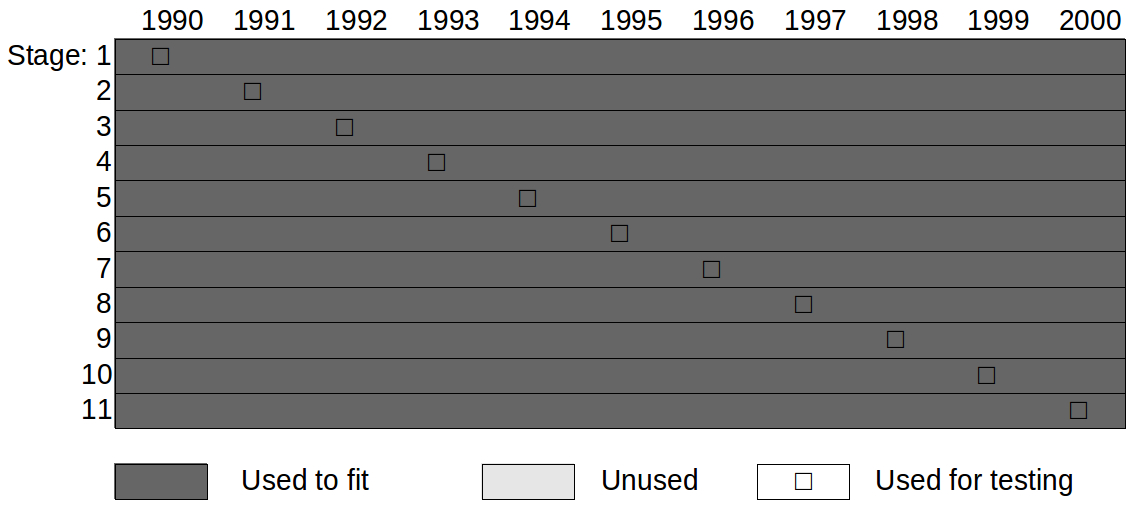
\includegraphics[width=\textwidth]{figures/raw/img-007.png}
  \caption{In sample back-testing: efficient but dishonest.\\
  样本内回测：高效，但不诚实。}
\end{figure}

In sample testing. You use all the data to fit and then test performance from the start. In
each stage (row) you test data for a different year, but use data from all years to fit.

\textit{样本内测试。你会先用全部数据完成拟合，然后从最早年份开始测试表现。
每一行代表你在测试某一个年份的数据，但拟合时使用的却始终是所有年份的数据。}

\begin{figure}[htbp]
  \centering
  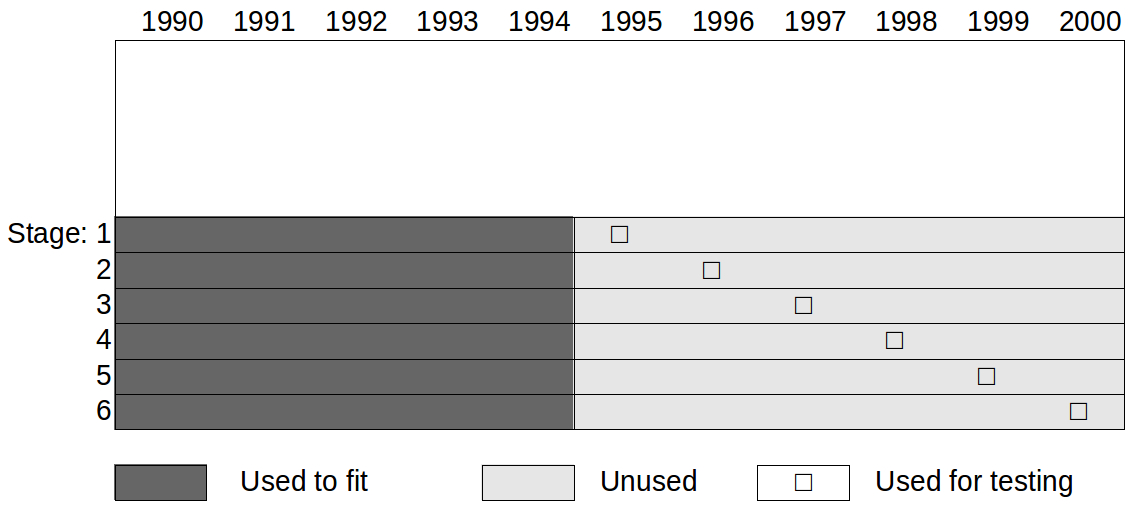
\includegraphics[width=\textwidth]{figures/raw/img-008.png}
  \caption{Half out of sample testing: honest, but wasteful.\\
  半样本外测试：诚实，但浪费数据。}
\end{figure}

You fit your trading rules on the first half, and then test performance on the second half.
In each stage (row) you test a different year, but always using the first half of the data to
fit. No testing is done in the first half of the data. The second half of the data isn't used
for fitting.

\textit{半样本外测试。你在前半段数据上拟合交易规则，然后在后半段数据上测试表现。
每一行都代表你测试其中某一个年份，但拟合时始终只使用前半段数据。
前半段不做测试，后半段不参与拟合。}

My preferred solution is to use an expanding window, as in figure
9.\footnote{This is sometimes called anchored fitting.\par 这有时也被称为 anchored fitting。} Suppose you think you need at least
a year to fit your system. In the next stage you fit on the first year of data for 1990, and
then test the resulting variation in the second year, 1991. Then in stage three of figure 9
you test in 1992 using the variation fitted with data from the years 1990 and 1991. To
test 1993 you use the best variation fitted using 1990, 1991 and 1992.

我最偏好的办法，
是使用扩张窗口，
也就是图 9 所示的方法。
假设你认为自己的系统至少需要一年的数据才能完成拟合。
那么在下一阶段，
你会先用 1990 这一整年的数据来拟合，
然后在第二年
--- 1991 年
--- 测试由此得到的变体。
接着在图 9 的第三阶段，
你会使用 1990 和 1991 两年的数据拟合出的变体，
去测试 1992 年。
同理，
如果你要测试 1993 年，
就应当使用基于 1990、1991 和 1992 三年数据拟合得到的最佳变体。

This continues until 2000 when you're using the previous ten years of data to select the
best variation. Because you only fit using the past you're not cheating. You also use as
much of the past as you ``legally'' can, so nothing is wasted.

这个过程会一直持续到 2000 年，
此时你会使用之前十年的数据来选择最佳变体。
由于你始终只使用过去已经发生的数据来拟合，
所以这并不算作弊。
与此同时，
你也“合法地”使用了尽可能多的历史数据，
因此几乎没有浪费。

The only problem with this method is that if the world changes you'll still be using
potentially irrelevant past data. To avoid this you could fit on the last five or ten years of
data, once you have enough history to do so, and discard earlier years. This is a rolling
window.\footnote{Another widely used term for this is walk forward fitting.\par 另一个常见术语是 walk forward fitting。} As figure 10
shows a five-year rolling window is identical to the expanding window until 1996. At this
point you would discard 1990, and use only the years 1991 to 1995 to fit the best
variation.

这种方法唯一的问题在于：
如果世界真的变了，
那你仍然会继续使用那些事实上已经不再相关的旧数据。
为了避免这一点，
一旦你的历史长度足够，
你就可以只用最近五年或十年的数据来拟合，
并把更早的数据丢掉。
这就是所谓的滚动窗口。
正如图 10 所展示的那样，
一个五年滚动窗口在 1996 年之前，
与扩张窗口其实是完全一样的。
到了 1996 年，
你才会把 1990 年丢掉，
仅使用 1991 到 1995 年来拟合最佳变体。

The length of the window needs to be short enough to pick up changes in market
structure, but long enough to give statistically significant results. As you'll see later you
often require multiple decades of data to fit models, which makes the use of rolling
windows problematic.

窗口的长度必须足够短，
才能及时捕捉市场结构的变化；
但同时又必须足够长，
才能给出具有统计显著性的结果。
而你稍后会看到，
拟合模型往往需要好几十年的数据，
这也正是为什么滚动窗口在实践中会变得很棘手。

\begin{figure}[htbp]
  \centering
  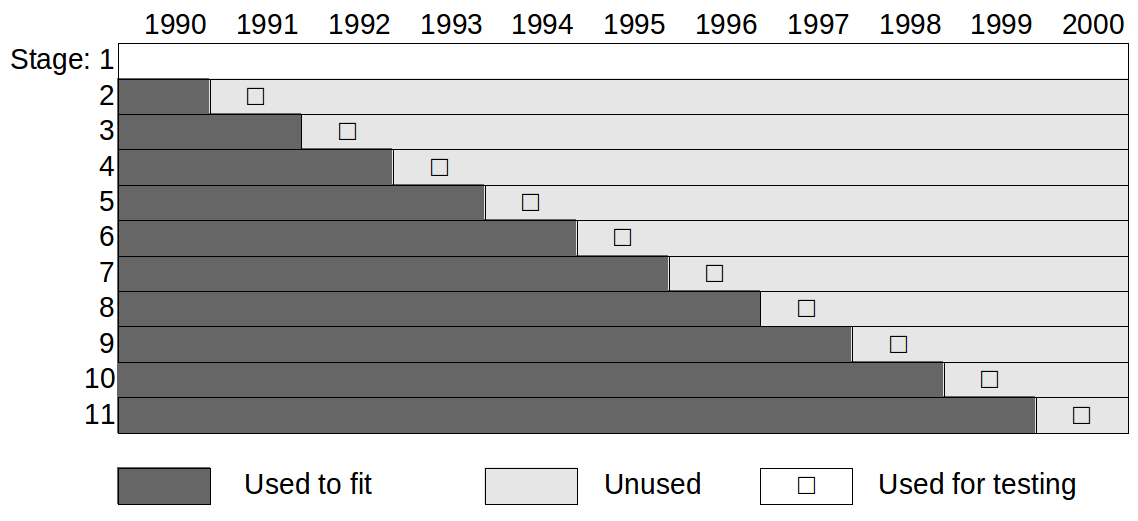
\includegraphics[width=\textwidth]{figures/raw/img-009.png}
  \caption{Expanding out of sample is both efficient and honest.\\
  扩张式样本外测试既高效又诚实。}
\end{figure}

Every year you fit the data only on the past. Each row shows the fitting and testing done
for a particular year.

\textit{扩张式样本外测试。每一年都只使用过去已经发生的数据来拟合。
每一行都展示了针对某一年的拟合与测试方式。}

\begin{figure}[htbp]
  \centering
  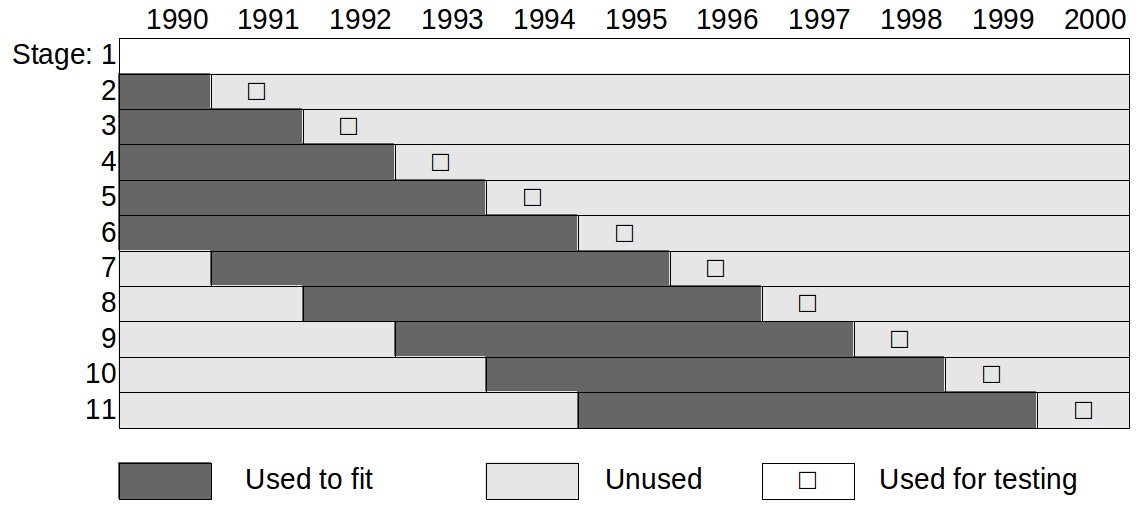
\includegraphics[width=\textwidth]{figures/raw/img-010.png}
  \caption{Rolling out of sample adapts to changing conditions, but make sure you have
  enough data for statistical significance.\\
  滚动样本外测试能适应变化，但你必须确保样本量足以支撑统计显著性。}
\end{figure}

Every year you use the past data to fit; up to five years' worth. Each row shows the
fitting and testing done for a particular year.

\textit{滚动样本外测试。每一年都用过去的数据拟合，但最多只回看五年。
每一行都展示了针对某一年的拟合与测试方式。}

\subsection*{When fitting goes bad}
\bisubsectiontitle{当拟合开始变坏时}

Now let's examine a concrete example of poor fitting practice. I'm going to select the best
variation of the early loss taker trading rule I introduced in chapter one to run over the
CME gold futures contract, out of a possible menu of 90 variations.\footnote{For those who
are interested this is based on the ``A and B'' system defined in appendix B. Values for B
(the stop loss value) will be the integers from 1 to 10; to capture different trend lengths.
Because I only want to look at trend following rules (early loss takers) I iterate only over
values of A (the profit target) that are equal to or larger than B: $A = 1 \times B$,
$1.5 \times B$, $2 \times B$, ... $5 \times B$. This gives 90 possible variations in all.\par 这个例子基于附录 B 中定义的 “A and B” 系统。
参数 B
（止损值）取 1 到 10 的整数，以覆盖不同趋势长度。
由于我这里只看趋势跟踪式规则
（也就是尽早止损者），
所以只遍历那些 A
（止盈目标）大于等于 B 的情况：
\(A = 1 \times B, 1.5 \times B, 2 \times B, \dots, 5 \times B\)。
总共有 90 个可能变体。}
This
might seem excessive, but it's fewer variations than Joe was testing in my earlier anecdote.
Bear in mind that if I had a five parameter trading rule, and I allowed each parameter to
take one of ten discrete values, then I'd be testing 10,000 variations!

现在让我们来看一个“糟糕拟合实践”的具体例子。
我准备从 90 个可能的变体中，
为第一章里介绍过的“尽早止损者”交易规则，
挑出在 CME 黄金期货上表现最好的那个变体。
这听起来已经很夸张了，
但仍然比前面故事里 Joe 测试过的变体数量还少。
别忘了，
如果我有一条五参数的交易规则，
并允许每个参数在十个离散取值中任选，
那么我实际上就在测试 10,000 个变体！

Once I have at least one year of data I find the highest performing variation based on the
Sharpe ratio (SR) from the previous 12 months. I then test the performance for the
following year, again using the last 12 months of data. This process is then repeated
annually. You should recognise this as a one year rolling window back-test.

Which of the following alternatives do you think will give me the best performance?

\begin{enumerate}
  \item Picking the best variation: Each year I use the best performing variation from the
  previous year.
  \item Picking a random variation: Ignoring my fitting, each year I choose one variation at
  random. Because the randomness of each choice will influence the results I run this
  experiment a number of times, and take the average performance.
  \item Keeping all the variations: Again ignoring my fitting, I keep all 90 variations, and
  use an equally weighted average of their forecasts.
\end{enumerate}

一旦我拥有至少一年的数据，
我就会根据过去 12 个月的夏普比率
（SR）
找出表现最好的那个变体。
随后，
我再使用过去 12 个月的数据，
去测试接下来一年的表现。
这一过程每年都会重复一次。
你应该能认出来，
这其实就是一个“一年滚动窗口”的回测。

那么，
你觉得下面哪一种做法会带来最佳表现？

1. 挑选最佳变体：
每年都使用上一年表现最好的那个变体。
2. 随机挑选变体：
完全无视拟合结果，
每年年初随机选一个变体。
由于随机选择本身会影响结果，
我会把实验重复很多次，
再取平均表现。
3. 保留全部变体：
同样无视拟合结果，
直接把 90 个变体全部保留下来，
并把它们的预测值做等权平均。

If you're a big fan of fitting the results are disappointing. Choosing the best rule each year
from the previous year gives me a rather poor SR of 0.07. If I go for the second option and
just choose a random rule annually each January 1st, then on average I get a Sharpe of
0.2. The best option is to forget about selecting trading rule variations entirely and run an
equal blend of them all. This gives an SR of 0.33, which is pretty good for one kind of
trading rule run on a single instrument. These results could be a fluke but I get similar
results on many different instruments and trading rules.

Why does fitting do so badly?

Firstly choosing just one variation to run at a time smacks of overconfidence. As you'll see
shortly we rarely have enough evidence that one rule is definitely better than another.
Secondly one year of data is wholly insufficient to decide which trading rule is best. I
make this problem worse by fitting on the history of a single instrument, gold futures.
Finally, like Joe, I am testing far too many variations.

如果你是拟合的忠实信徒，
那结果会令人非常失望。
如果每年都选择“上一年表现最好的规则”，
我得到的 SR 居然只有可怜的 0.07。
如果我换成第二种做法，
也就是每年 1 月 1 日随机挑一条规则，
那么平均下来还能得到 0.2 的 Sharpe。
而最好的做法，
竟然是彻底忘掉“挑规则变体”这件事，
直接把 90 个变体全部保留下来并等权混合。
这样一来，
SR 居然能达到 0.33，
对于单一品种上运行的一类交易规则来说，
这已经相当不错了。
这些结果当然有可能只是巧合，
但我在许多不同品种和不同交易规则上都得到了类似结论。

为什么拟合会表现得这么糟糕呢？

这里我给出一个拟合走偏的具体例子：
我从 90 个可能变体中，
去为 CME 黄金期货挑选“尽早止损者”规则里表现最好的那一个变体。
这听起来已经很多了，
但你别忘了，
它仍然比前面故事里 Joe 测试过的规则数量还少。
如果我有一条五参数规则，
而每个参数都能取十个离散值，
那么我就已经在测试 10,000 个变体了。

接着我采用一年滚动窗口：
只要拥有至少一年数据，
我就用过去 12 个月里夏普比率最高的变体，
来测试接下来的一年。
然后每年都重复这个过程。

问题是：
你猜哪种方法表现最好？
1. 每年都选上一年最好的变体；
2. 完全随机地选一个变体；
3. 什么都不挑，把 90 个变体全部保留下来，然后等权平均。

结果很残酷：
每年都挑“上一年最好的那个”，
反而只得到大约 0.07 的夏普；
每年随机挑一个，
平均下来大约是 0.2；
最好的办法居然是压根别选，
而是把 90 个变体全部等权组合起来，
夏普反而有 0.33。

也就是说，
拟合在这里不但没有帮你，
反而害了你。
原因很简单：
第一，
每次只押注一个变体，
本身就充满过度自信；
第二，
一年数据远远不足以判断哪条规则真的更好；
第三，
我测试的变体数量本来就太多了。

\subsection*{The hazards of rule selection}
\bisubsectiontitle{规则筛选的风险}

\subsubsection*{The multiple testing problem --- even some random rules will look good}

Why is it so dangerous to test large numbers of trading rules and variations? Apart from
the effort involved it's very likely that you will end up picking a poor rule just by chance.

To see why here is an experiment. Let's suppose I am trying to achieve alchemy and find
profitable rules where there are none to be had. I have a pool of a certain number of
possible trading rules, all of which have true expected average returns of zero, although in
a real scenario I wouldn't know this beforehand! The rules are entirely arbitrary and their
returns are generated from random data.\footnote{Many of the examples in this chapter
will use imaginary daily returns of various arbitrary trading rule variations. These fake
returns are randomly generated with the kind of characteristics I want: expected mean,
standard deviation (from which we get the Sharpe ratio), and where relevant correlation
with other variations. I then run these tests many times and report the average result, so
the answer is not influenced by how each series of random numbers come out.\par 本章中很多例子都会使用人为生成的“假”日收益序列。
这些收益是随机生成的，
但会满足我所设定的特征：
给定的均值、
标准差
（从而决定夏普比率），
以及必要时与其他变体之间的相关性。
我会把这些实验重复很多次，
再报告平均结果，
这样结论就不会被某一次具体随机数的偶然结果所左右。}

For each test I get one year of return data for each rule in my pool, as in the gold futures
example above, and select all the rules whose Sharpe ratio (SR) in that year is higher than
a given minimum level. If no rule has an SR above the threshold then I won't choose any.
All the rules that pass the test will be kept (even if there are 50!).

Because the underlying data is random I need to generate new data multiple times and then
repeat the test to get meaningful results. I then measure the average number of rules
accepted given a specific minimum level and the size of the pool available. As table 3
shows, even if I'm strict and set an extremely high minimum SR of 2.0 I'll still pick up a
couple of bad rules if I test enough of them.

为什么大规模测试交易规则和变体会如此危险？
除了你得付出大量劳动之外，
更大的风险在于：
你最后极有可能只是靠运气，
就挑中了一条很差的规则。

要理解这一点，
我们来看一个实验。
假设我想在根本不存在盈利机会的地方，
通过某种炼金术硬是找出赚钱规则。
我手里有一个由若干可能规则组成的规则池，
而这些规则的真实预期平均收益全都等于零，
只是现实里我事先并不知道这一点。
这些规则完全是任意构造的，
它们的收益也全都来自随机数据。

在每次测试里，
我都会像前面黄金期货的例子那样，
为规则池中的每一条规则生成一年的收益数据，
然后挑出那些在这一年里夏普比率
（SR）
高于某个最低门槛的规则。
如果没有任何规则高于这个阈值，
那我就一个都不选。
所有通过检验的规则都会被保留下来
--- 哪怕最后通过的有 50 条！

由于底层数据是随机的，
我必须不断生成新数据并重复这个测试，
结果才有意义。
随后，
我再根据给定的最小门槛和规则池大小，
去测量平均会有多少条规则被接受。
正如表 3 所示，
即便我非常严格，
把最低 SR 门槛设到离谱的 2.0，
只要测试的规则足够多，
我最终还是会捞出几条坏规则。

\begin{table}[htbp]
  \centering
  \small
  \caption{If you test enough rules, some bad ones will always slip through\\
  如果你测试足够多的规则，总会有一些坏规则混进来}
  \begin{tabular}{@{}lccc@{}}
    \toprule
    Number of rules tested in pool & 0.5 & 1.0 & 2.0 \\
    \midrule
    1 & $<1$ & $<1$ & $<1$ \\
    5 & 1.4 & $<1$ & $<1$ \\
    10 & 3 & 1.5 & $<1$ \\
    50 & 16 & 8 & 1.2 \\
    100 & 30 & 16 & 2.3 \\
    \bottomrule
  \end{tabular}
\end{table}

The table shows the average number of rules accepted from pools of arbitrary unprofitable
rules, given different pool sizes (rows), which were tested to see if their Sharpe ratio
exceeded a minimum cutoff (columns).

Practically then what SR cutoff should I use? As none of the imaginary rules are truly
profitable ideally I wouldn't accept any. But in real fitting situations we can't set the bar
too high or even good rules will be discarded; after all a realistic SR for a real trading rule,
tested on one instrument, is only likely to be around 0.30. Let's suppose I would be happy
with a 5\% chance of picking out at least one rule that was truly unprofitable. Also in the
real world I'd usually have more than one year of data, so let's see what effect additional
history has on my findings.

Table 4 has all the results. As you might have suspected the length of the return series is
very important here. More history means less chance of a zero SR rule getting a lucky
streak, so I can set the cutoff lower. However, even with 30 years of data I can't risk
testing more than a handful of rules, and even then the cutoff is far too high when many
perfectly good variations will only have true Sharpe ratios of 0.3.

\begin{table}[htbp]
  \centering
  \small
  \caption{With more history you can set a lower Sharpe ratio threshold to avoid picking a
  bad rule from a larger pool\\
  如果历史数据更多，你可以把夏普阈值设得更低，同时减少从大规则池里挑中坏规则的概率}
  \begin{tabular}{@{}lcccc@{}}
    \toprule
    Number of rules tested & 1 & 5 & 10 & 30 \\
    \midrule
    1 & 1.5 & 0.7 & 0.5 & 0.4 \\
    5 & 2.3 & 1.1 & 0.8 & 0.5 \\
    10 & 2.8 & 1.2 & 0.8 & 0.6 \\
    50 & 3.4 & 1.5 & 1.0 & 0.6 \\
    100 & 3.4 & 1.5 & 1.1 & 0.7 \\
    \bottomrule
  \end{tabular}
\end{table}

The table shows the Sharpe ratio cutoff needed when testing a given size pool (rows) of
trading rules, with a certain amount of years of historical data (columns) to ensure you
only have a 5\% chance of picking out one or more truly bad rules.

\subsubsection*{How much history do you need to decide if a rule is good?}

You've now seen that a common mistake is to use insufficient historical data to select or
calibrate a rule. How much data do you need? How long do you need to decide if a rule
has a positive Sharpe ratio (SR) and is worth keeping?

To answer this I generated more random trading rule daily returns, this time assuming an
underlying positive Sharpe ratio, which again I wouldn't know in advance. As more
trading history is generated I can estimate the SR each year and the average so far. At the
same time I look at the distribution of those annual Sharpe ratios.\footnote{For a more
technical discussion of this issue, see Andrew Lo's paper ``The Statistics of Sharpe ratios''
in \textit{Financial Analysts Journal} 58:4, July/August 2002.} This allows me to get a feel
for how statistically significant my measured average SR is; was I just lucky or is this really
a good system?

A classic test for statistical significance is the T-Test. In this example it determines
whether an estimated Sharpe ratio is likely to be positive given the estimate of its mean and
standard deviation. The further away the mean is from zero, as measured in units of
sigma, the more likely the unknown SR is actually positive.

This test is commonly used with a threshold of two sigma. If an estimated average SR is
more than two standard deviations above zero there would only be a 2.5\% chance of this
happening if the true SR was actually negative.

Figure 11 shows the evolution of the average measured SR for an arbitrary trading rule,
and around it the upper and lower ``confidence intervals''. Each confidence interval is two
sigma away from the average, so when the lower interval pushes above zero I know there
is only a 2.5\% chance the trading system is really a loss making rule in disguise.

\begin{figure}[htbp]
  \centering
  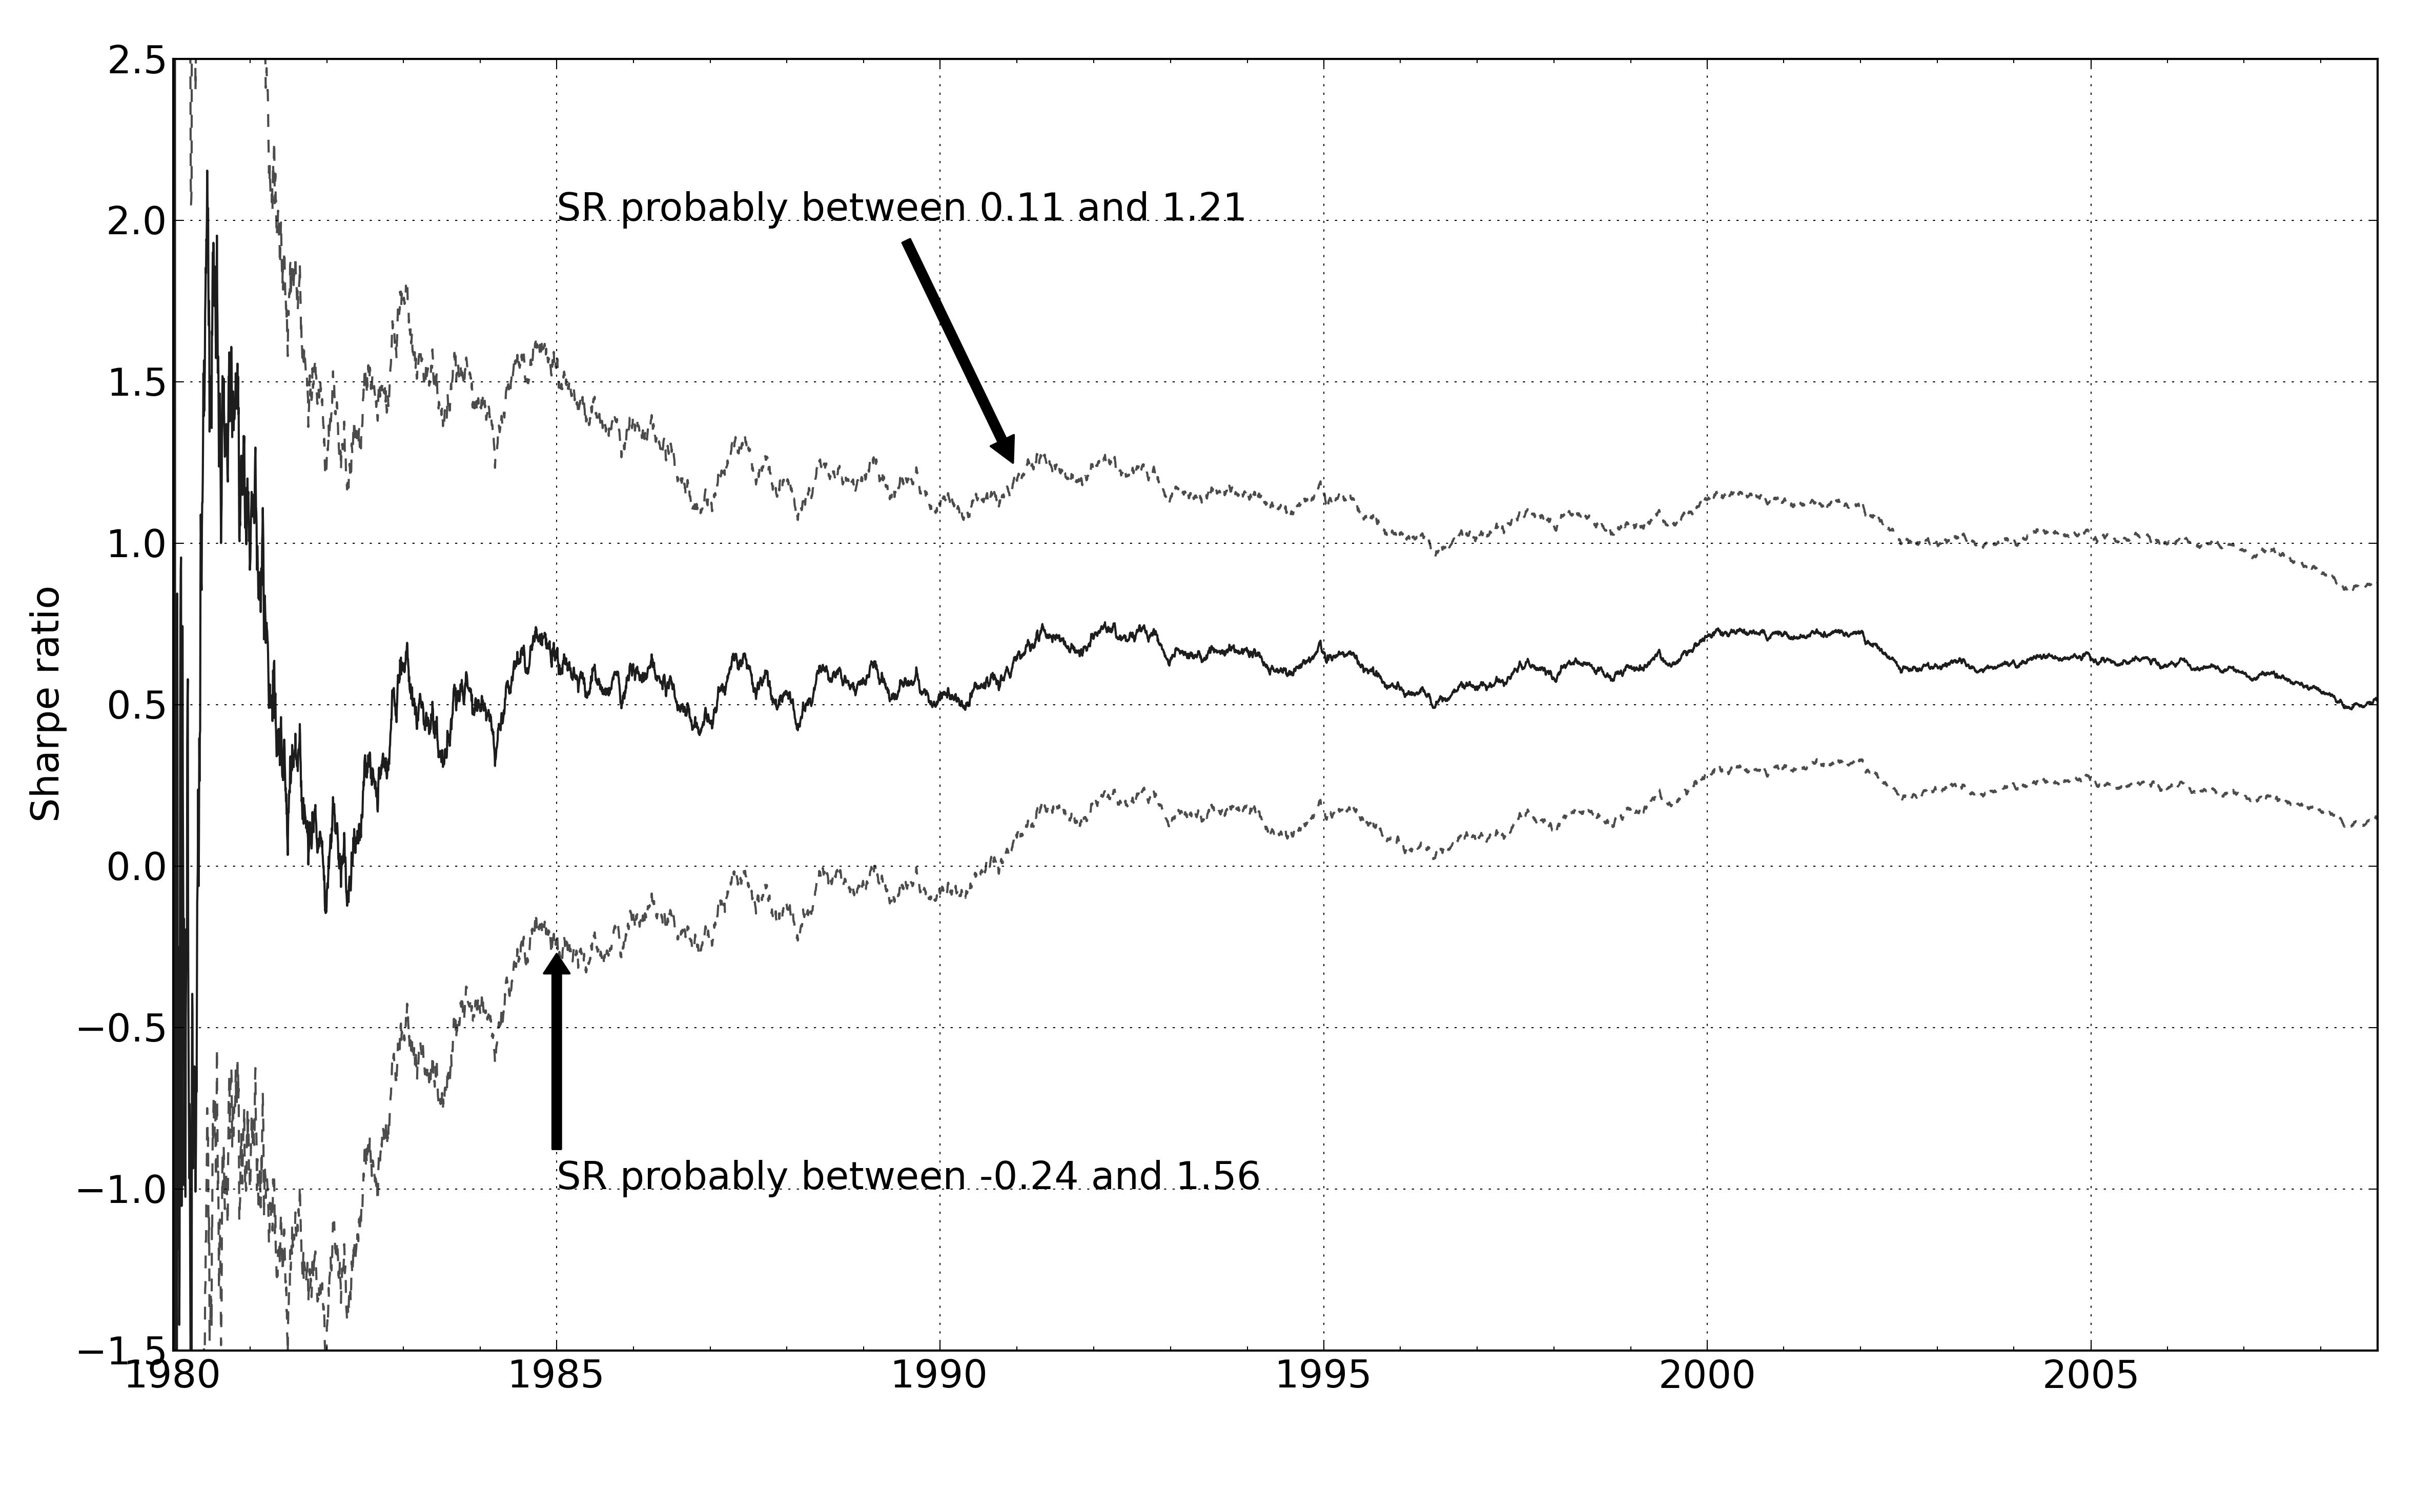
\includegraphics[width=\textwidth]{figures/raw/img-011.png}
  \caption{With a true Sharpe ratio (SR) of 0.5, it takes more than ten years to pass the
  T-Test and conclude the SR is probably positive.}
\end{figure}

In the figure you can see the average SR converging quickly on the true value of 0.5 SR.
But it takes over ten years before the lower confidence interval goes above zero and the
T-Test is finally passed. Only then can we be reasonably certain this is not a loss making
system.

If I repeat this for a rule with a true SR of 1.0 I get figure 12. The time to pass the test
here is just a few years. On average it will always take less time for higher SR strategies to
prove their profitability.

\begin{figure}[htbp]
  \centering
  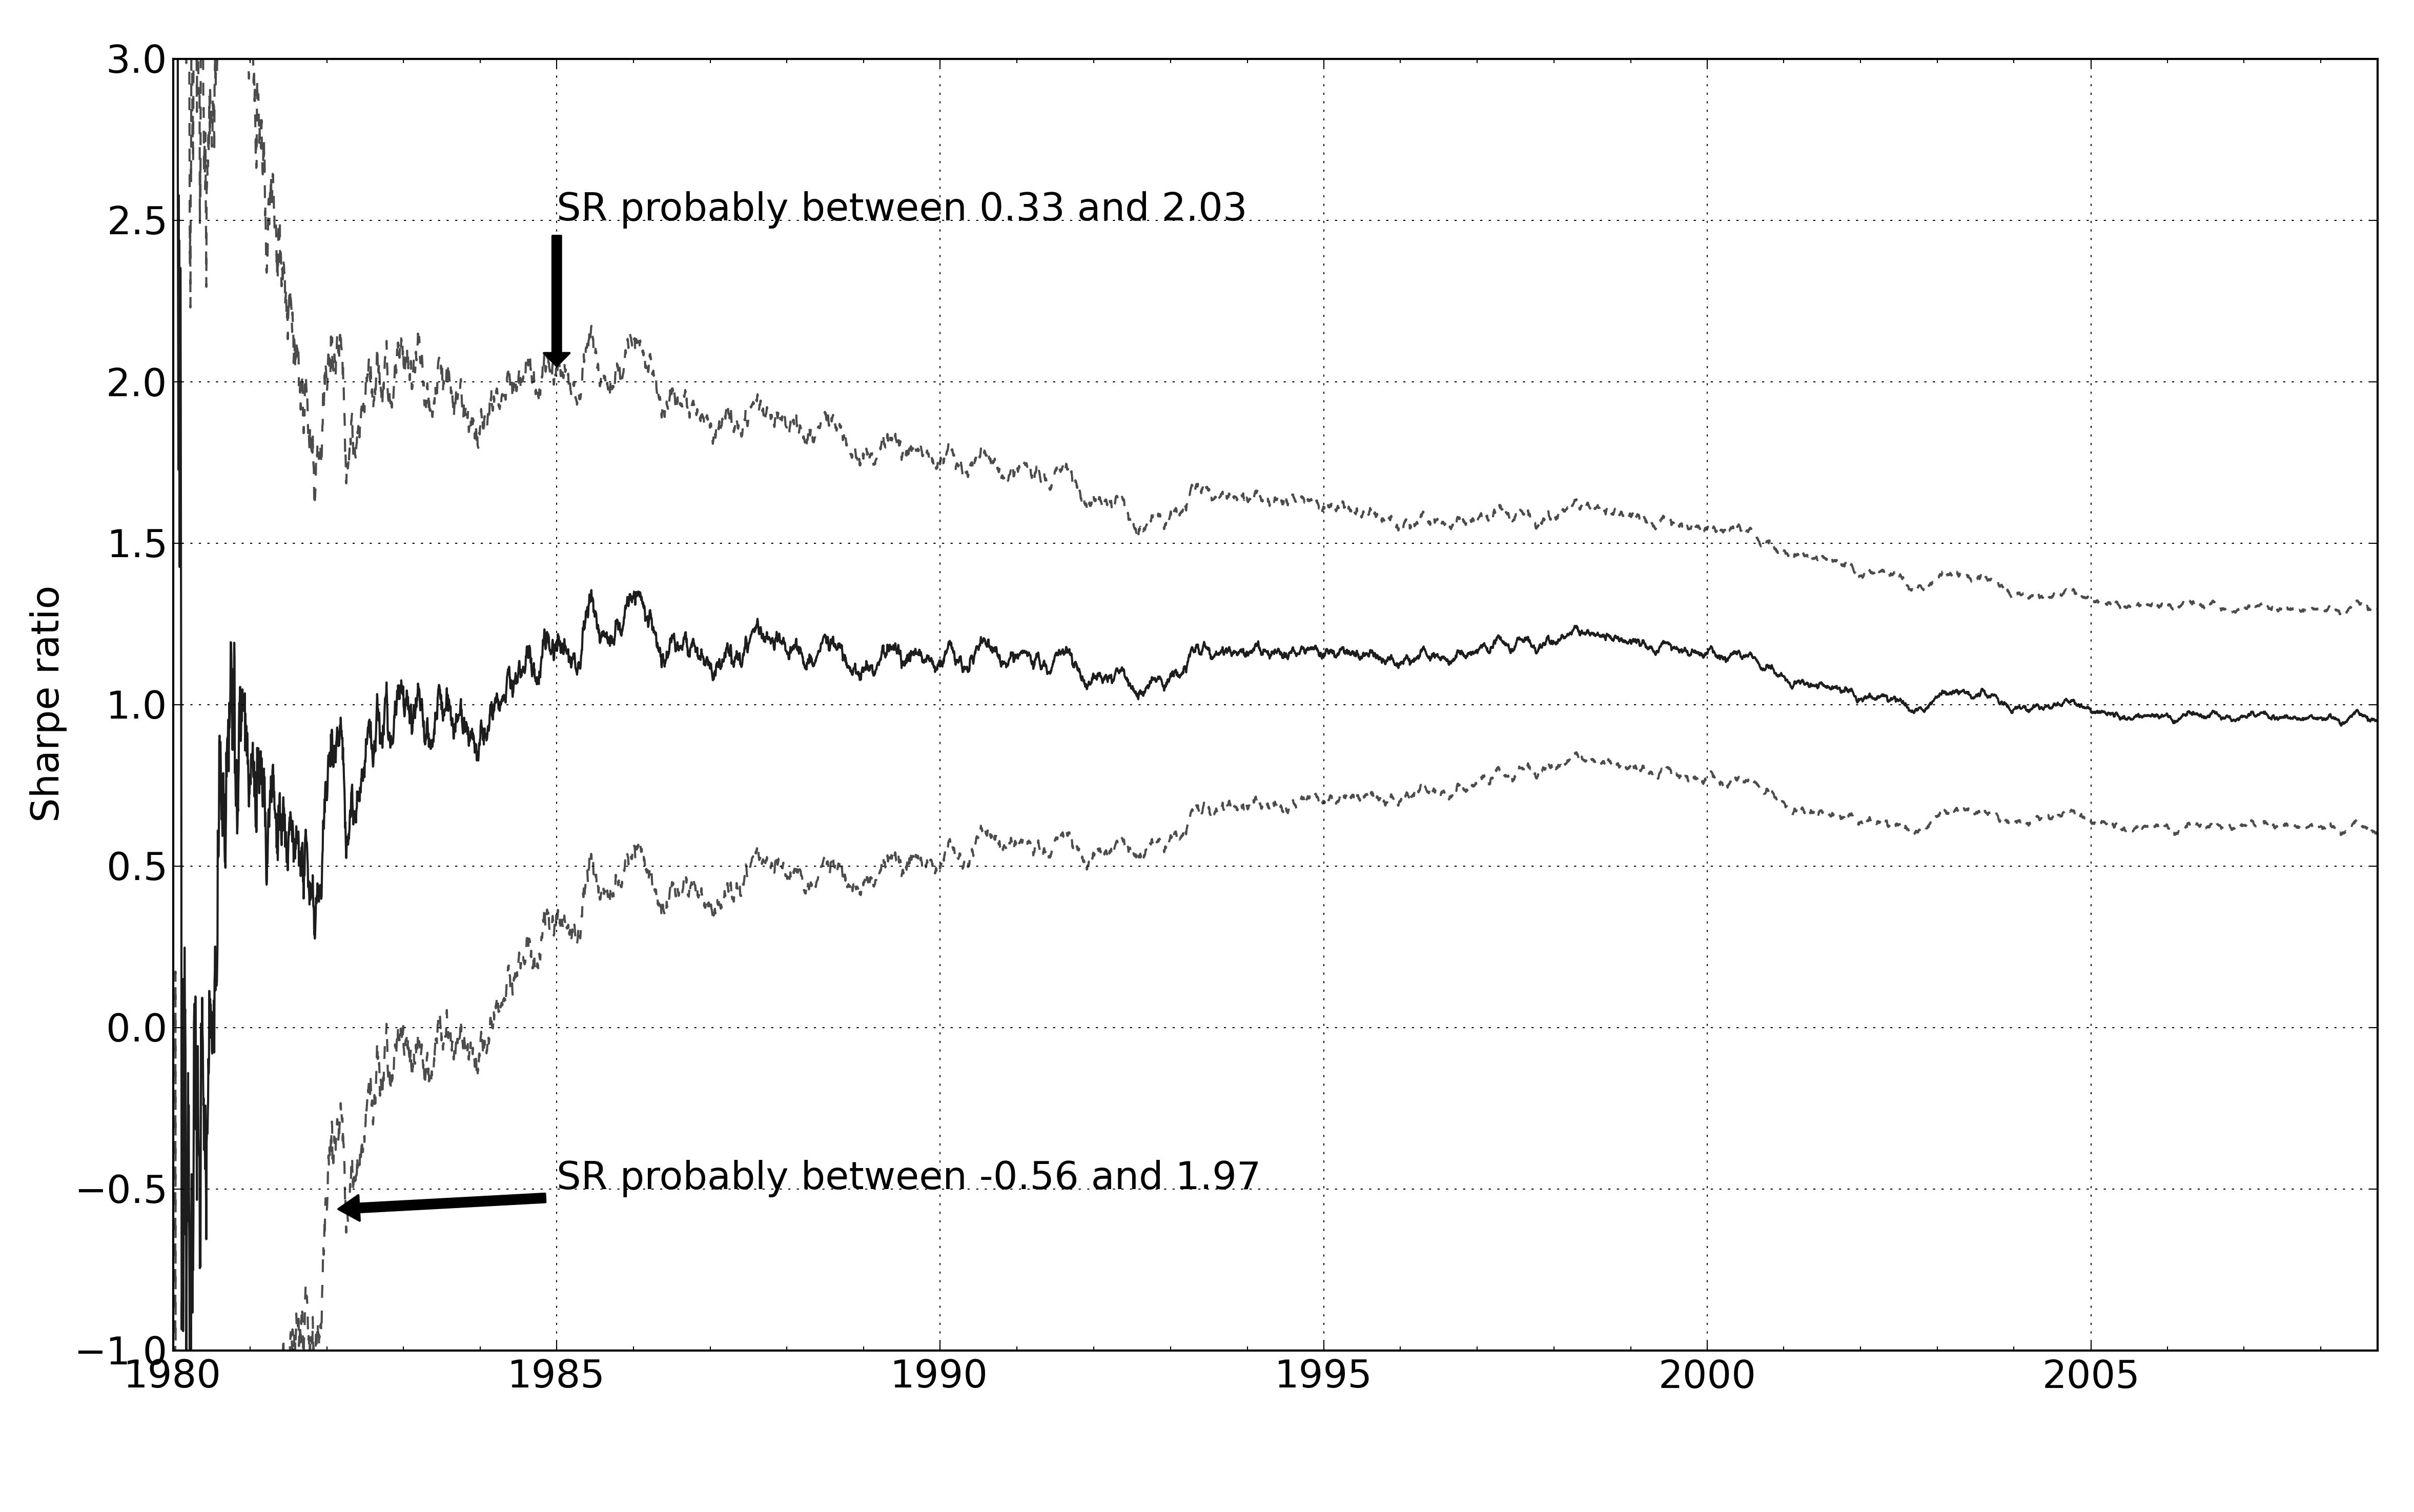
\includegraphics[width=\textwidth]{figures/raw/img-012.png}
  \caption{With a true Sharpe ratio of 1.0 we pass the T-Test in a few years.}
\end{figure}

Let's find the average time to pass the test for a given true Sharpe ratio. After running the
necessary experiments I get table 5. Except for very good rules you need at least ten years,
and usually more, to be sure a strategy makes money.\footnote{These results also depend
on the skew of returns. For example, with a true SR of 1.0 I needed about three years'
more data for a typical negative skew volatility selling strategy to pass the T-Test,
compared to a positive skew trend following strategy.} The average trading rule for one
instrument has a realistic SR of around 0.3; so you'd need nearly 40 years of history!

\begin{table}[htbp]
  \centering
  \small
  \caption{It takes decades of data to see if most strategies are likely to be profitable\\
  对大多数策略而言，要判断其是否真正可能盈利，往往需要几十年的数据}
  \begin{tabular}{@{}lcccccccc@{}}
    \toprule
    True Sharpe ratio & 0.2 & 0.3 & 0.4 & 0.5 & 0.7 & 1.0 & 1.5 & 2.0 \\
    Average years to pass profit T-Test & 45 & 37 & 33 & 20 & 10 & 6 & 3 & 1.4 \\
    \bottomrule
  \end{tabular}
\end{table}

The table shows average time in years to pass the T-Test for profitability given the true
Sharpe ratio of the trading rule.

\subsubsection*{How much history do you need to decide if one rule is better than another?}

Now what if you have some alternative rules and want to find the best. Let's suppose I
again have two random rules, one with a true Sharpe ratio (SR) of 0.30, and the other an
SR of 0.80. Initially I'm going to assume these are quite different rules with no correlation
between their returns. This time to perform the T-Test I need to estimate the difference in
the two Sharpe ratios, and measure the average and standard deviation of that difference.

\begin{figure}[htbp]
  \centering
  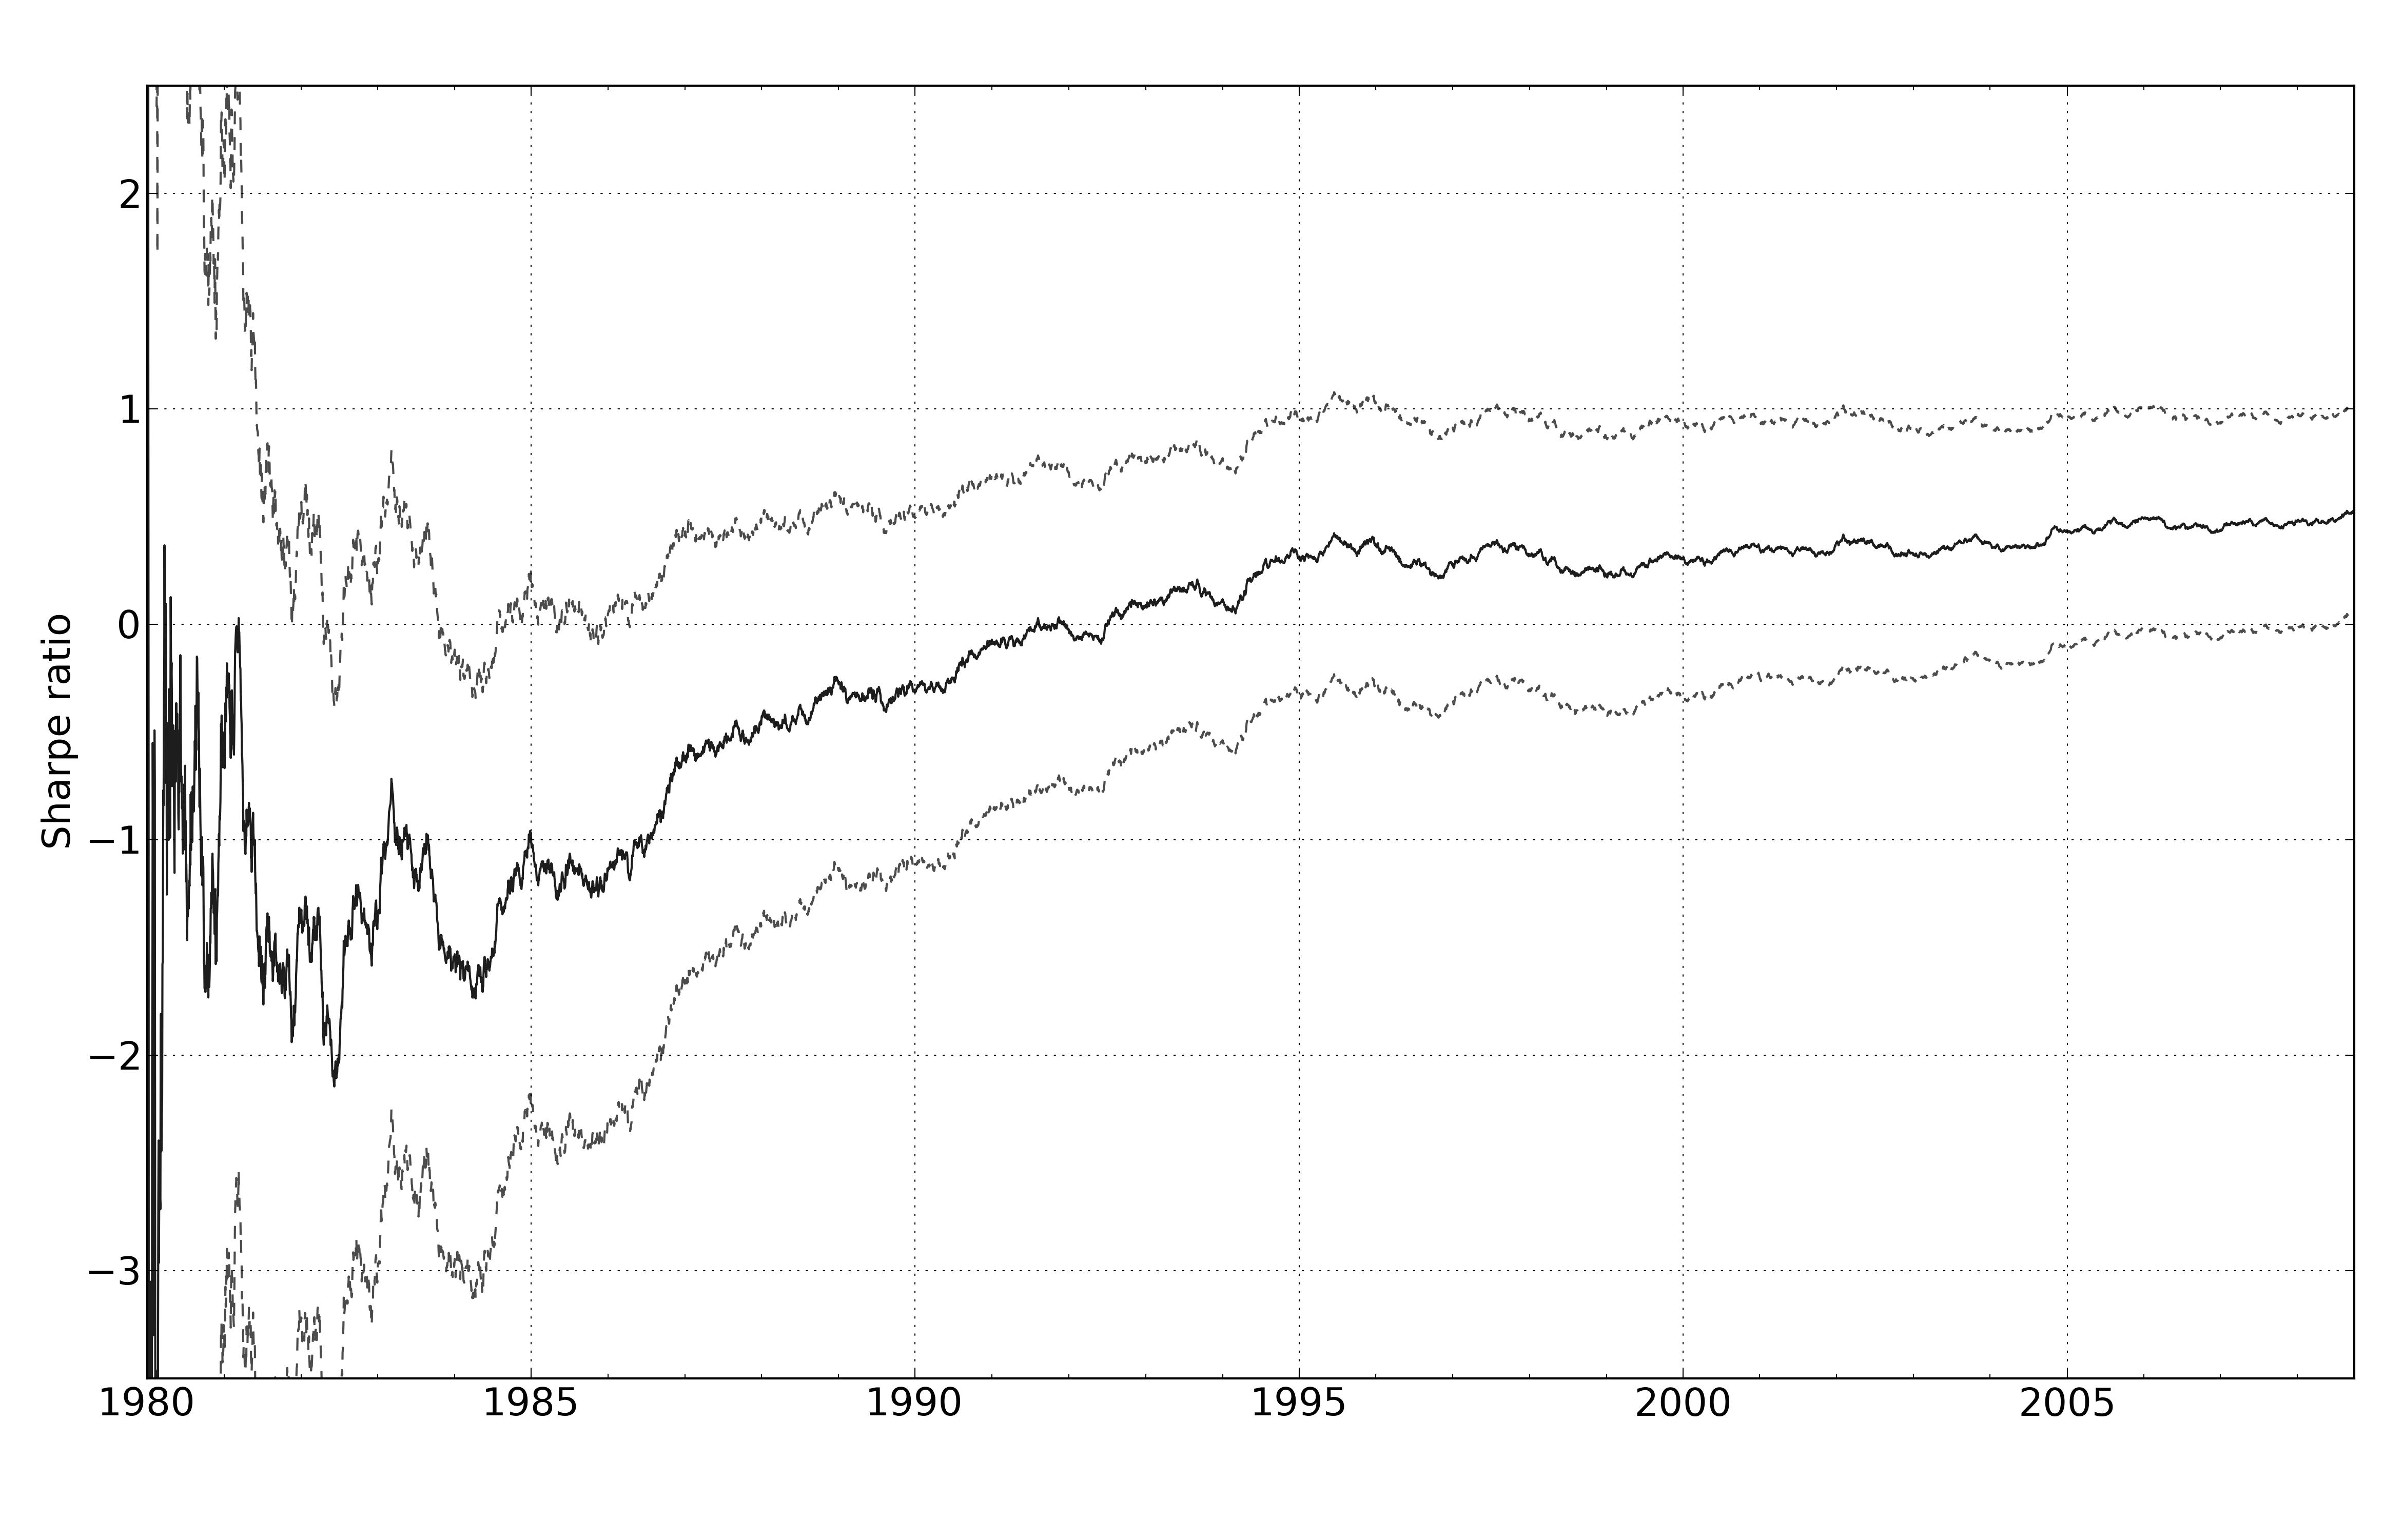
\includegraphics[width=\textwidth]{figures/raw/img-013.png}
  \caption{It takes three decades to discover that this SR 0.8 strategy is probably better
  than an uncorrelated strategy with SR 0.3.}
\end{figure}

In figure 13 is the average difference in SR and the relevant confidence intervals for this
difference. Once the lower confidence interval goes above zero then we can be reasonably
certain that one rule is better, as again there is only a 2.5\% probability of this happening
by chance. You can see from figure 13 that the time to certainty is around 30 years!

Table 6 shows the average time taken to pass the T-Test when comparing an SR 0.30 rule
with one that truly has a higher SR. These results vary depending on the difference in SR
and the correlation of the rules. More closely related rules will be easier and quicker to
distinguish for a given SR difference.\footnote{More subtly the overall level of the Sharpes
involved will also influence the results, as Andrew Lo's paper discusses. The skew of the
rules is also important, even when comparing rules with similar skew.} In practice
distinguishing rules requires considerable historical data except for the rare cases of
variations which are both highly correlated, and also perform very differently.

\begin{table}[htbp]
  \centering
  \small
  \caption{Can you distinguish trading rules given a few years of data? Only if they are
  highly correlated and one heavily outperforms the other\\
  只凭几年数据，你能区分规则优劣吗？只有在规则高度相关且其中一个明显优于另一个时才有可能}
  \begin{tabular}{@{}lccccc@{}}
    \toprule
    Sharpe ratio advantage & -1.0 & 0.0 & 0.5 & 0.8 & 0.95 \\
    \midrule
    0.1 & 47 & 47 & 46 & 44 & 37 \\
    0.25 & 46 & 45 & 40 & 32 & 10 \\
    0.5 & 41 & 37 & 25 & 10 & 3 \\
    1.0 & 23 & 11 & 8 & 2.5 & 0.5 \\
    \bottomrule
  \end{tabular}
\end{table}

The table shows the number of years needed for us to be reasonably certain that one rule
is better than another, given the SR advantage of the better rule (rows) and the correlation
between the trading returns of the two rules (columns).

为什么大规模测试会这么危险？
因为哪怕所有规则本质上都没有任何盈利能力，
只要你测试得足够多，
总会有一些“看起来很棒”的规则幸运混出来。

上面的几张表说明了几个核心事实：
1. 规则池越大，
你越容易误选出坏规则。
2. 历史样本越长，
你才越有资格把“筛选阈值”放低一些。
3. 即便一条规则真的有正的夏普比率，
要在统计意义上证明它大概是正的，
通常也需要非常多年。
4. 若你想证明规则 A 比规则 B 更好，
所需数据比证明“一条规则不是垃圾”还要更多。

直白一点说，
大多数时候，
你根本没有足够的数据，
去理直气壮地说：
“这一条规则明显优于那一条。”

\subsubsection*{Should you fit one trading rule for all instruments?}

In 2010 the large systematic hedge fund in which I worked was reorganised into asset
classes. My team managed the fixed income portfolio, another ran equities and so on.
Initially the trading strategies we ran were fairly similar. However over time, as we did
more market specific research, we all became convinced that we needed to customise our
systems differently.

In many cases we went further and also began to fit different parts of our portfolios
separately. We might for example have fitted emerging and developed market bond
futures with different trading rule variations.\footnote{In reality we didn't do this. Or did
we? Unfortunately I can't give real examples without breaking the terms of my
non-disclosure agreement.\par 现实中我们并没有这么做。或者说，做过吗？
很遗憾，我不能举真实例子，
否则就会违反保密协议。} Fitting separately is common, and many system traders take
this to the extreme and fit every instrument separately. Almost all back-testing packages,
such as the one Joe was using, default to fitting trading rules on a single instrument at a
time. So you would have one variation of a rule for the British pound/dollar, another for
euro/dollar and so on.

This is a classic example of the narrative fallacy, a cognitive bias we have seen before. To
our human minds it makes sense to have different stories, and so different trading rules,
for different instruments.

But is this the right thing to do? It depends on whether the behaviour of each variation
over the various instruments is significantly different. If it isn't then you're likely to be
over-fitting by individually tailoring each rule for every instrument. In practice there isn't
usually a statistical difference between different instruments, particularly if they are closely
related such as a group of equity index futures.\footnote{There are some exceptions,
notably when there are different trading costs for the instruments concerned, which I'll
cover in chapter twelve, ``Speed and Size''.\par 当然也有例外，
尤其是当不同工具的交易成本差异很大时，
这一点我会在第十二章“速度与规模”中讨论。}

In fact pooling your data and fitting multiple instruments together is an excellent way of
getting more data history, which gives you a better shot at being able to distinguish
profitable and loss making trading rules.

As an example I have two trading rules in my own portfolio which for a typical single
instrument have Sharpe ratios (SR) averaging 0.05 and 0.30 respectively. Despite being
perfectly uncorrelated, table 6 shows I'd need 45 years to distinguish them; almost
impossible when even the earliest financial futures only began trading in 1972. However
the same rules run on a portfolio of instruments have SR of 0.13 and
1.13.\footnote{Technical note: These are the returns you'd get if you traded an equally
weighted portfolio of instruments using the same trading rule. The improvement in Sharpe
ratio (SR) comes from the diversification effect across instruments. The alternative method
is to stitch consecutive series of instrument returns together. This gives a very long history
of returns, but the SR of the stitched series will be almost the same as the average across
individual instruments (it is not identical to the average because of the effect of varying
lengths of price series for different instruments).} The table shows I'd need just 11 years
of data to distinguish these two Sharpe ratios from each other.

To make pooling easier you should design trading rules that are generic and can work with
any instrument. I'll give some examples of generic rules in chapter seven, ``Forecasts''.

2010 年，
我所在的大型系统化对冲基金按资产类别进行了重组。
我的团队负责固定收益投资组合，
另一支团队负责股票，
其他团队也各自管理不同板块。
最开始，
我们运行的交易策略还算比较相似。
但随着大家做了越来越多针对具体市场的研究，
我们都逐渐相信：
自己的系统需要被分别定制。

在很多情况下，
我们甚至更进一步，
开始把投资组合中的不同部分也分别拿出来拟合。
例如，
我们完全可能会为新兴市场债券期货和发达市场债券期货，
分别拟合不同的交易规则变体。
这种“分开拟合”的做法很常见，
而许多系统交易者会把它推到极端，
对每一个品种都单独拟合。
几乎所有回测软件
--- 比如 Joe 当时所用的那类
--- 默认也都是一次只针对单一品种拟合交易规则。
于是，
英镑兑美元会有一种规则变体，
欧元兑美元会有另一种，
其余品种也都各自为政。

这正是叙事谬误的经典例子，
而我们之前已经见识过这种认知偏差。
对人类大脑来说，
给不同品种讲不同故事，
于是再给它们配上不同的交易规则，
听上去非常合理。

但这样做真的是对的吗？
答案取决于：
每个变体在不同品种上的行为，
是否真的存在显著差异。
如果没有，
那你很可能只是在通过“给每个品种单独量身定做规则”的方式进行过拟合。
而在现实中，
不同品种之间通常并不存在统计上显著的差异，
尤其是当它们彼此非常接近时，
例如一组股票指数期货。

事实上，
把多个品种的数据合并起来一起拟合，
是获得更多历史样本的极佳方式。
这样一来，
你更有机会区分哪些交易规则真正能赚钱，
哪些只是会亏钱的噪声。

为了让这种“合并数据”更容易实现，
你应当设计通用型交易规则，
让它们能够适用于任何品种。
我会在第七章“预测值”中给出一些这类通用规则的例子。

另一个常见错误，是把每个品种都单独拟合出一套专属规则。
这在直觉上很诱人，
因为人类喜欢给不同市场讲不同故事。
但问题在于：
除非你能证明不同品种上的规则行为真的存在显著差异，
否则这种“量身定做”通常就是过拟合。

现实里，
尤其是在那些彼此非常相近的品种
（例如一组股指期货）之间，
这种显著差异通常很难被统计地证明。
与其把每个品种分开拟合，
不如把多个品种的数据合并起来，
这样反而能得到更多历史样本，
也更有机会区分规则究竟是赚钱，
还是只是噪声。

\section*{Some rules for effective fitting}
\phantomsection
\addcontentsline{toc}{section}{Some rules for effective fitting}
\bisectiontitle{有效拟合的一些规则}

If you haven't been warned off fitting, and insist on using data to select and calibrate
trading rules, then following this advice should keep you out of serious trouble. Those who
are now rightly terrified of fitting can skip ahead to the next section, where I show you
how I avoid fitting almost completely.

如果你在经历了前面的警告之后，
仍然坚持要用数据来选择和校准交易规则，
那么遵循下面这些建议，
至少可以让你避免掉进最严重的坑里。
如果你现在已经被拟合吓得足够警觉，
那也完全可以直接跳到下一节，
在那里我会告诉你，
我是如何几乎完全绕开拟合的。

\subsection*{Keep it simple}
\bisubsectiontitle{保持简单}

I am not a fan of complex fitting methods and I prefer not to use them. But if you do
consider yourself an expert in a dark statistical art then naturally you would want to
practise it. Just be aware; the more complex the method the harder it will be to realise
when you are over-fitting.

我并不喜欢复杂的拟合方法，
也更倾向于不用它们。
但如果你自认是某种黑暗统计艺术的专家，
那你当然会想去施展它。
只是请记住：
方法越复杂，
你就越难意识到自己什么时候已经过拟合了。

\subsection*{Fewer alternatives}
\bisubsectiontitle{减少候选项}

As table 4 shows reducing the pool of trading rules and variations considered is crucial
unless you have many years of data.\footnote{If you are using a more complex fitting
technique then you need to keep your degrees of freedom appropriately small.\par 如果你使用的是更复杂的拟合技术，
那么你也必须把自由度控制得足够低。}

正如表 4 所展示的那样，
除非你真的拥有很多很多年的数据，
否则减少候选交易规则与变体的数量，
就是重中之重。

\subsection*{Ban time machines}
\bisubsectiontitle{禁止使用时光机}

You should always use rolling or expanding out of sample fitting. If using a rolling
window don't make it too short; be aware of the number of years needed to distinguish
rules from random noise, and each other (tables 4, 5 and 6).

你应当始终使用滚动式或扩张式样本外拟合。
如果你采用的是滚动窗口，
就不要把窗口设得太短。
一定要清楚：
想要把一条规则和随机噪声区分开来，
以及把规则彼此区分开来，
到底需要多少年的数据
（见表 4、表 5 和表 6）。

\subsection*{Don't drop rules casually}
\bisubsectiontitle{不要轻率淘汰规则}

Before picking one rule or variation and discarding others based on past performance, look
carefully at table 6. It's unusual in reality to find highly correlated rules with radically
different performance. More likely you will find very different rules with perhaps a Sharpe
ratio (SR) difference of 0.5 but almost no correlation, or highly correlated rule variations
which are very similar in SR. In both cases you need 30 years of data to differentiate them.
It's rare to have 30 years or more of price history, so it's difficult to justify picking one rule
over another on performance alone.

在你根据过去表现挑出一条规则、
同时把其他规则丢掉之前，
请先认真看看表 6。
现实中，
高度相关但表现天差地别的规则其实并不常见。
你更可能看到的是：
两条非常不同的规则，
夏普比率也许差了 0.5，
但几乎没有相关性；
或者若干高度相关的规则变体，
它们的 SR 又非常接近。
而在这两种情形下，
你通常都需要 30 年的数据，
才能把它们区分开来。
问题是，
现实里很少有人真的拥有 30 年以上的价格历史，
所以单凭表现去偏爱某一条规则，
往往很难自圆其说。

\subsection*{Pool data across instruments}
\bisubsectiontitle{跨品种合并数据}

You're going to need all the data you can to make good fitting decisions. The easiest
solution is to pool data from multiple instruments.

Only if there is a statistically significant difference in performance between various rules
across instruments should you fit them individually. In practice this is rarely necessary.

想要做出好的拟合决策，
你需要尽可能多的数据。
最简单的办法，
就是把多个品种的数据合并起来。

只有当不同规则在不同品种上的表现差异，
在统计意义上真的显著时，
你才应该分别拟合它们。
而在现实中，
这种情况其实很少见。

\subsection*{Compare apples with apples}
\bisubsectiontitle{拿可比的东西做比较}

I've assumed throughout this chapter that you will use Sharpe ratio (SR) to compare rules.
But comparing a positively skewed rule and a negatively skewed alternative purely on SR is
highly misleading, as negative skew rules will tend to have flatteringly high SR.

整章里我都默认，
你会用夏普比率
（SR）
来比较规则。
但如果你只是机械地用 SR 去比较一条正偏度规则和一条负偏度规则，
那会非常误导。
因为负偏度规则往往会拥有一种“看起来很漂亮”的高 SR。

\subsection*{When the future won't be like the past}
\bisubsectiontitle{当未来不会像过去那样时}

Be careful of focusing on outright performance, rather than returns relative to benchmarks.
This is very dangerous because many asset classes, like equities and bonds, have done
extraordinarily well over the last 40 years or so. The easiest way to get extra back-tested
profits is to use trading rules which are more highly correlated with the underlying asset
class.

This is unlikely to work in the future as the main cause of these high returns was
significant falls in inflation; something that won't be repeated.

要小心，
不要只盯着绝对表现，
而忽视相对于基准的收益。
这非常危险，
因为过去大约 40 年里，
许多资产类别
--- 比如股票和债券
--- 的表现都异常优秀。
而想要轻松“做高回测利润”的最简单方法，
就是去使用那些和底层资产类别本身高度相关的交易规则。

但这种做法未来很可能行不通，
因为过去那些高收益最主要的原因之一，
是通胀的大幅下行；
而这件事不太可能再发生一次。

如果你无论如何都要拟合，
那么至少要遵守几条底线：
1. 方法保持简单；
2. 候选规则和变体尽可能少；
3. 永远使用扩张式或滚动式样本外拟合；
4. 不要因为一点点表现差异就轻易淘汰规则；
5. 尽量跨品种合并数据；
6. 比较规则时，
要比较真正可比的对象；
7. 不要把过去那个异常好的宏观时代，
误当成未来也会重复出现的常态。

\section*{How I choose my rules}
\phantomsection
\addcontentsline{toc}{section}{How I choose my rules}
\bisectiontitle{我如何选择自己的规则}

There are many ways to navigate the fitting minefield. My own preference is to avoid it
almost completely, by selecting trading rules and variations without looking at actual
performance. I use the following process:

要穿过拟合这片雷区，
方法有很多。
而我个人更偏好的办法，
是几乎完全绕开它：
在选择交易规则和变体时，
尽量不去看它们的真实历史表现。
我使用的是下面这样一个流程：

\begin{enumerate}
  \item Come up with a small number of trading rules to exploit each idea I have about
  how the market behaves.
  \item For each rule select a few variations. At this stage I am not looking at performance,
  but at behaviour such as trading speed and correlation with other variations.
  \item Allocate forecast weights to each variation, taking uncertainty about Sharpe ratios
  into account. Poor rules will have lower weight, but are rarely entirely excluded.
\end{enumerate}

This process means that I don't use performance to fit trading rules and variations. Instead
returns data is reserved for finding forecast weights. These weights determine in what
proportion each variation is used to predict each instrument's returns. The next chapter
will explain how this portfolio allocation can reduce the weight on apparently poor
variations without risking over-fitting.

Any variation that ends up with a negligible weight in the final portfolio can ultimately be
dropped from your live trading system, reducing the complexity of implementation. This
gives the same end result as excluding the rule earlier, but it means any back-tested
performance incorporating the excluded rule will be more realistic.

这一流程意味着：
我不会用历史表现去拟合交易规则和它们的变体。
相反，
收益数据会被保留到后面，
专门用来决定预测权重。
这些权重会决定：
每个变体在多大程度上被用来预测每个品种的收益。
下一章会解释，
这种组合配置过程如何在不引发过拟合风险的前提下，
降低那些看起来较差的变体权重。

任何一个最终在投资组合中权重已经低到几乎可以忽略的变体，
最后都可以从你的实盘系统里删除，
从而降低实现复杂度。
这在结果上，
与更早把那条规则排除掉是一样的；
但它能让包含该规则的回测表现显得更真实。

\subsection*{Start with a small number of ideas}
\bisubsectiontitle{从少量想法开始}

I prefer to come up with a relatively small number of ideas for trading rules. In my own
portfolio I have eight rules drawn from five different themes, but if I was starting from
scratch I'd begin with just a couple of rules: the trend following and carry rules that I will
show you in chapter seven, ``Forecasts''.

You should have a small number of rules because:

\begin{enumerate}
  \item Less risk of over-fitting: Fewer ideas means less chance of over-fitting, and a lower
  critical Sharpe ratio is required before accepting a rule (table 4).
  \item Many ways to skin the feline: One kind of market behaviour can be picked up in
  multiple ways. For example we can capture trends with momentum oscillators,
  divergence and breakout systems to name but a few. There is little value in having
  dozens of similar rules for one kind of behaviour.
  \item Keep it simple: With my process all the rules will survive the selection process so
  starting with too many rules will create complexity in the trading system. Complex
  systems are more difficult to trust and understand.
\end{enumerate}

Far too much time and effort is spent by both amateur and professional trading system
designers in looking for more, and better, trading rules. But the marginal value of adding
additional rules is low, especially if they are of the same trading style. The average
correlation between different rules trading a particular instrument is higher than between
instruments trading the same rule. So diversification amongst instruments is preferable to
rule diversification.

Adding new instruments is a tiresome task of uploading and checking data which is less
fun than coming up with more trading rules, but in my experience is of far more benefit.

我倾向于只提出相对较少数量的交易规则想法。
在我自己的投资组合里，
我一共使用八条规则，
它们来自五种不同主题；
但如果让我从零开始，
我大概只会先从两条规则起步：
也就是我将在第七章“预测值”中展示的趋势跟随和 carry 规则。

你之所以应该只保留少量规则，
原因有三：

1. 过拟合风险更低：
想法越少，
过拟合的机会就越低，
而在接受一条规则前所需要达到的临界夏普比率也会更低
（见表 4）。
2. 同一种市场行为有很多种捕捉方式：
例如，
趋势可以通过动量振荡器、背离系统、突破系统等多种方式被捕捉。
为同一种市场行为准备几十条相似规则，
其实没有太大价值。
3. 保持简单：
按照我的流程，
这些规则最终大多都会保留下来。
如果一开始规则太多，
那你的交易系统就会变得异常复杂。
而复杂系统更难以信任，
也更难以理解。

无论是业余还是专业的交易系统设计者，
都花了太多时间和精力在“寻找更多、更好规则”这件事上。
但增加额外规则的边际价值其实很低，
尤其是当这些规则属于同一种交易风格时。
对于某个特定品种来说，
不同规则之间的平均相关性，
通常高于“同一条规则在不同品种之间”的相关性。
因此，
来自“品种分散化”的收益，
通常优于“规则分散化”。

增加新工具这件事，
无非是上传与检查数据，
做起来远没有想新规则那么有趣。
但根据我的经验，
它带来的收益却往往大得多。

\subsection*{Keep the right number of variations}
\bisubsectiontitle{保留合适数量的变体}

Although I prefer to have relatively few trading rules I wouldn't normally have just one
variation of any rule which can be calibrated. But there is no need to use 90 or more
possible combinations! For example if you're trying to capture price momentum then you
will probably need a variation that captures relatively fast trends, one that captures very
slow moves and perhaps two to three in between.

If two of your variations have more than a 95\% correlation you can safely drop one of
them since it will have almost no marginal benefit. You can also remove variations whose
trading costs will be too high, or which trade extremely slowly and so are unlikely to give
you significant returns. But do not drop variations purely because of their performance.

虽然我偏好规则数量尽量少，
但对于那些可以校准的规则，
我通常也不会只保留一个单独变体。
不过，
这绝不意味着你需要保留 90 个甚至更多组合！
例如，
如果你想捕捉价格动量，
那么你大概只需要一个捕捉较快趋势的变体、
一个捕捉很慢运动的变体，
以及夹在中间的两到三个变体。

如果你的两个变体之间相关性已经高于 95\%，
那你完全可以安全地删掉其中一个，
因为它几乎不会带来任何边际收益。
你也可以删除那些交易成本过高的变体，
或者那些慢得离谱、
几乎不可能贡献显著收益的变体。
但千万不要仅仅因为表现不佳，
就把某个变体删掉。

\subsection*{Don't look at returns - yet}
\bisubsectiontitle{先别看收益}

My preference is to reserve actual historic performance data for deciding which forecast
weights to give to trading rules and their variations. Done properly this can give you
realistic back-tested performance and still down-weight poor trading rules. But if you've
already used real data to pre-select only good rules then your back-test performance will
be too optimistic, and you'll have over-fitted.

So at this stage it's only behaviour such as correlation and likely trading costs you should
be looking at, not performance. You must avoid contaminating the back-test.

There isn't much detail about this process here but there will be examples of how it works
later in the book. Whether you fit your trading rules, or use my hands off approach, the
next problem is to decide how much of rule X and how much of Y --- and how much of
instrument A or B --- to use in your trading system. This problem of portfolio allocation is
covered in the next chapter.

我的偏好是：
把真实历史表现数据保留到最后，
只用它来决定该给各条交易规则及其变体分配多少预测权重。
如果操作得当，
这既可以让你的回测表现更现实，
又仍然能降低那些较差交易规则的权重。
但如果你已经提前用真实数据把“好规则”筛出来了，
那你的回测表现就一定会过于乐观，
而你也就已经过拟合了。

所以在这一阶段，
你应该看的只是行为特征，
例如相关性和大致交易成本，
而不是表现本身。
你必须避免污染回测。

这里我没有展开太多细节，
但书后面会给出这一流程如何运作的例子。
无论你是选择去拟合交易规则，
还是采用我这种更“放手”的方式，
下一步你都必须面对同一个问题：
在自己的交易系统里，
规则 X 应该占多少，
规则 Y 又该占多少，
而品种 A 和品种 B 又该分配多大比例？
这个“组合配置”的问题，
就是下一章要讨论的主题。

我的方法可以概括成三步：
1. 先从少量、彼此差异清晰的市场想法开始；
2. 每条规则只保留少数几个真正有行为差异的变体，
而不是堆一大堆；
3. 在真正决定权重之前，
尽量不要看历史收益表现，
而只关注相关性、
交易速度和成本等行为特征。

这样做的关键点在于：
我不把“历史表现”拿来筛选规则，
而是把它保留给后面用于分配预测权重。
结果是，
差一点的规则会被减权，
但不会因为一点看似差的表现就被过早淘汰。
等到最终组合里某个变体权重已经低到可以忽略时，
你当然可以在实盘里把它去掉，
这样既降低实现复杂度，
也能让整个回测结果比“先删后测”更真实。
